% Options for packages loaded elsewhere
\PassOptionsToPackage{unicode}{hyperref}
\PassOptionsToPackage{hyphens}{url}
\PassOptionsToPackage{dvipsnames,svgnames,x11names}{xcolor}
%
\documentclass[
  11pt,
]{article}

\usepackage{amsmath,amssymb}
\usepackage{iftex}
\ifPDFTeX
  \usepackage[T1]{fontenc}
  \usepackage[utf8]{inputenc}
  \usepackage{textcomp} % provide euro and other symbols
\else % if luatex or xetex
  \usepackage{unicode-math}
  \defaultfontfeatures{Scale=MatchLowercase}
  \defaultfontfeatures[\rmfamily]{Ligatures=TeX,Scale=1}
\fi
\usepackage{lmodern}
\ifPDFTeX\else  
    % xetex/luatex font selection
  \setmainfont[]{Latin Modern Roman}
  \setmathfont[]{Latin Modern Math}
\fi
% Use upquote if available, for straight quotes in verbatim environments
\IfFileExists{upquote.sty}{\usepackage{upquote}}{}
\IfFileExists{microtype.sty}{% use microtype if available
  \usepackage[]{microtype}
  \UseMicrotypeSet[protrusion]{basicmath} % disable protrusion for tt fonts
}{}
\makeatletter
\@ifundefined{KOMAClassName}{% if non-KOMA class
  \IfFileExists{parskip.sty}{%
    \usepackage{parskip}
  }{% else
    \setlength{\parindent}{0pt}
    \setlength{\parskip}{6pt plus 2pt minus 1pt}}
}{% if KOMA class
  \KOMAoptions{parskip=half}}
\makeatother
\usepackage{xcolor}
\setlength{\emergencystretch}{3em} % prevent overfull lines
\setcounter{secnumdepth}{5}
% Make \paragraph and \subparagraph free-standing
\ifx\paragraph\undefined\else
  \let\oldparagraph\paragraph
  \renewcommand{\paragraph}[1]{\oldparagraph{#1}\mbox{}}
\fi
\ifx\subparagraph\undefined\else
  \let\oldsubparagraph\subparagraph
  \renewcommand{\subparagraph}[1]{\oldsubparagraph{#1}\mbox{}}
\fi

\usepackage{color}
\usepackage{fancyvrb}
\newcommand{\VerbBar}{|}
\newcommand{\VERB}{\Verb[commandchars=\\\{\}]}
\DefineVerbatimEnvironment{Highlighting}{Verbatim}{commandchars=\\\{\}}
% Add ',fontsize=\small' for more characters per line
\usepackage{framed}
\definecolor{shadecolor}{RGB}{241,243,245}
\newenvironment{Shaded}{\begin{snugshade}}{\end{snugshade}}
\newcommand{\AlertTok}[1]{\textcolor[rgb]{0.68,0.00,0.00}{#1}}
\newcommand{\AnnotationTok}[1]{\textcolor[rgb]{0.37,0.37,0.37}{#1}}
\newcommand{\AttributeTok}[1]{\textcolor[rgb]{0.40,0.45,0.13}{#1}}
\newcommand{\BaseNTok}[1]{\textcolor[rgb]{0.68,0.00,0.00}{#1}}
\newcommand{\BuiltInTok}[1]{\textcolor[rgb]{0.00,0.23,0.31}{#1}}
\newcommand{\CharTok}[1]{\textcolor[rgb]{0.13,0.47,0.30}{#1}}
\newcommand{\CommentTok}[1]{\textcolor[rgb]{0.37,0.37,0.37}{#1}}
\newcommand{\CommentVarTok}[1]{\textcolor[rgb]{0.37,0.37,0.37}{\textit{#1}}}
\newcommand{\ConstantTok}[1]{\textcolor[rgb]{0.56,0.35,0.01}{#1}}
\newcommand{\ControlFlowTok}[1]{\textcolor[rgb]{0.00,0.23,0.31}{#1}}
\newcommand{\DataTypeTok}[1]{\textcolor[rgb]{0.68,0.00,0.00}{#1}}
\newcommand{\DecValTok}[1]{\textcolor[rgb]{0.68,0.00,0.00}{#1}}
\newcommand{\DocumentationTok}[1]{\textcolor[rgb]{0.37,0.37,0.37}{\textit{#1}}}
\newcommand{\ErrorTok}[1]{\textcolor[rgb]{0.68,0.00,0.00}{#1}}
\newcommand{\ExtensionTok}[1]{\textcolor[rgb]{0.00,0.23,0.31}{#1}}
\newcommand{\FloatTok}[1]{\textcolor[rgb]{0.68,0.00,0.00}{#1}}
\newcommand{\FunctionTok}[1]{\textcolor[rgb]{0.28,0.35,0.67}{#1}}
\newcommand{\ImportTok}[1]{\textcolor[rgb]{0.00,0.46,0.62}{#1}}
\newcommand{\InformationTok}[1]{\textcolor[rgb]{0.37,0.37,0.37}{#1}}
\newcommand{\KeywordTok}[1]{\textcolor[rgb]{0.00,0.23,0.31}{#1}}
\newcommand{\NormalTok}[1]{\textcolor[rgb]{0.00,0.23,0.31}{#1}}
\newcommand{\OperatorTok}[1]{\textcolor[rgb]{0.37,0.37,0.37}{#1}}
\newcommand{\OtherTok}[1]{\textcolor[rgb]{0.00,0.23,0.31}{#1}}
\newcommand{\PreprocessorTok}[1]{\textcolor[rgb]{0.68,0.00,0.00}{#1}}
\newcommand{\RegionMarkerTok}[1]{\textcolor[rgb]{0.00,0.23,0.31}{#1}}
\newcommand{\SpecialCharTok}[1]{\textcolor[rgb]{0.37,0.37,0.37}{#1}}
\newcommand{\SpecialStringTok}[1]{\textcolor[rgb]{0.13,0.47,0.30}{#1}}
\newcommand{\StringTok}[1]{\textcolor[rgb]{0.13,0.47,0.30}{#1}}
\newcommand{\VariableTok}[1]{\textcolor[rgb]{0.07,0.07,0.07}{#1}}
\newcommand{\VerbatimStringTok}[1]{\textcolor[rgb]{0.13,0.47,0.30}{#1}}
\newcommand{\WarningTok}[1]{\textcolor[rgb]{0.37,0.37,0.37}{\textit{#1}}}

\providecommand{\tightlist}{%
  \setlength{\itemsep}{0pt}\setlength{\parskip}{0pt}}\usepackage{longtable,booktabs,array}
\usepackage{calc} % for calculating minipage widths
% Correct order of tables after \paragraph or \subparagraph
\usepackage{etoolbox}
\makeatletter
\patchcmd\longtable{\par}{\if@noskipsec\mbox{}\fi\par}{}{}
\makeatother
% Allow footnotes in longtable head/foot
\IfFileExists{footnotehyper.sty}{\usepackage{footnotehyper}}{\usepackage{footnote}}
\makesavenoteenv{longtable}
\usepackage{graphicx}
\makeatletter
\def\maxwidth{\ifdim\Gin@nat@width>\linewidth\linewidth\else\Gin@nat@width\fi}
\def\maxheight{\ifdim\Gin@nat@height>\textheight\textheight\else\Gin@nat@height\fi}
\makeatother
% Scale images if necessary, so that they will not overflow the page
% margins by default, and it is still possible to overwrite the defaults
% using explicit options in \includegraphics[width, height, ...]{}
\setkeys{Gin}{width=\maxwidth,height=\maxheight,keepaspectratio}
% Set default figure placement to htbp
\makeatletter
\def\fps@figure{htbp}
\makeatother
\newlength{\cslhangindent}
\setlength{\cslhangindent}{1.5em}
\newlength{\csllabelwidth}
\setlength{\csllabelwidth}{3em}
\newlength{\cslentryspacingunit} % times entry-spacing
\setlength{\cslentryspacingunit}{\parskip}
\newenvironment{CSLReferences}[2] % #1 hanging-ident, #2 entry spacing
 {% don't indent paragraphs
  \setlength{\parindent}{0pt}
  % turn on hanging indent if param 1 is 1
  \ifodd #1
  \let\oldpar\par
  \def\par{\hangindent=\cslhangindent\oldpar}
  \fi
  % set entry spacing
  \setlength{\parskip}{#2\cslentryspacingunit}
 }%
 {}
\usepackage{calc}
\newcommand{\CSLBlock}[1]{#1\hfill\break}
\newcommand{\CSLLeftMargin}[1]{\parbox[t]{\csllabelwidth}{#1}}
\newcommand{\CSLRightInline}[1]{\parbox[t]{\linewidth - \csllabelwidth}{#1}\break}
\newcommand{\CSLIndent}[1]{\hspace{\cslhangindent}#1}

\usepackage{booktabs}
\usepackage{longtable}
\usepackage{arxiv}
\usepackage{orcidlink}
\usepackage{amsmath}
\usepackage[T1]{fontenc}
\makeatletter
\makeatother
\makeatletter
\makeatother
\makeatletter
\@ifpackageloaded{caption}{}{\usepackage{caption}}
\AtBeginDocument{%
\ifdefined\contentsname
  \renewcommand*\contentsname{Table of contents}
\else
  \newcommand\contentsname{Table of contents}
\fi
\ifdefined\listfigurename
  \renewcommand*\listfigurename{List of Figures}
\else
  \newcommand\listfigurename{List of Figures}
\fi
\ifdefined\listtablename
  \renewcommand*\listtablename{List of Tables}
\else
  \newcommand\listtablename{List of Tables}
\fi
\ifdefined\figurename
  \renewcommand*\figurename{Figure}
\else
  \newcommand\figurename{Figure}
\fi
\ifdefined\tablename
  \renewcommand*\tablename{Table}
\else
  \newcommand\tablename{Table}
\fi
}
\@ifpackageloaded{float}{}{\usepackage{float}}
\floatstyle{ruled}
\@ifundefined{c@chapter}{\newfloat{codelisting}{h}{lop}}{\newfloat{codelisting}{h}{lop}[chapter]}
\floatname{codelisting}{Listing}
\newcommand*\listoflistings{\listof{codelisting}{List of Listings}}
\makeatother
\makeatletter
\@ifpackageloaded{caption}{}{\usepackage{caption}}
\@ifpackageloaded{subcaption}{}{\usepackage{subcaption}}
\makeatother
\makeatletter
\@ifpackageloaded{tcolorbox}{}{\usepackage[skins,breakable]{tcolorbox}}
\makeatother
\makeatletter
\@ifundefined{shadecolor}{\definecolor{shadecolor}{rgb}{.97, .97, .97}}
\makeatother
\makeatletter
\makeatother
\makeatletter
\makeatother
\ifLuaTeX
  \usepackage{selnolig}  % disable illegal ligatures
\fi
\IfFileExists{bookmark.sty}{\usepackage{bookmark}}{\usepackage{hyperref}}
\IfFileExists{xurl.sty}{\usepackage{xurl}}{} % add URL line breaks if available
\urlstyle{same} % disable monospaced font for URLs
\hypersetup{
  pdftitle={Quantitative Risk Assessment of Bitcoin's Proof-of-Work Security Model},
  pdfauthor={Ingo Giebel},
  pdfkeywords={Bitcoin, Proof-of-Work, mining economics, hashrate
concentration, censorship resistance, institutional risk, content
pollution, Ordinals, ETF compliance, Almgren-Chriss, difficulty
adjustment},
  colorlinks=true,
  linkcolor={blue},
  filecolor={Maroon},
  citecolor={blue},
  urlcolor={blue},
  pdfcreator={LaTeX via pandoc}}

\renewcommand{\today}{2026-02-01}
\newcommand{\runninghead}{A Preprint }
\title{Quantitative Risk Assessment of Bitcoin's Proof-of-Work Security
Model}
\def\asep{\\\\\\ } % default: all authors on same column
\author{\textbf{Ingo
Giebel}~\orcidlink{0009-0005-4238-000X}\\\\Independent Researcher\\\\}
\date{2026-02-01}
\begin{document}
\maketitle
\begin{abstract}
We present a quantitative framework for assessing systemic risks in
Bitcoin's Proof-of-Work (PoW) security model through four interconnected
simulation models. Our analysis examines (1) miner capitulation dynamics
under price stress with difficulty adjustment feedback, (2) blockchain
content pollution via Ordinals and OP\_RETURN abuse with fee-market
dampening, (3) hashrate concentration and censorship resistance, and (4)
institutional exit cascades triggered by compliance concerns using
Almgren-Chriss optimal execution modeling. Results indicate critical
vulnerabilities: a Nakamoto Coefficient of only 3, content pollution
approaching \textasciitilde40\% saturation (down from earlier estimates
after incorporating fee-market dynamics), and a potential institutional
exit cascade scenario. Additionally, the growing trend of Bitcoin miners
pivoting to AI/HPC hosting (e.g., TeraWulf with Google Cloud, Core
Scientific with CoreWeave) introduces a structural shift in miner
economics that reduces hashrate concentration risk while increasing the
vulnerability of pure-play BTC miners. These findings suggest that
Bitcoin's security guarantees may be more fragile than commonly assumed,
though endogenous stabilization mechanisms (difficulty adjustment, fee
markets) provide meaningful resilience.
\end{abstract}
{\bfseries \emph Keywords}
\def\sep{\textbullet\ }
Bitcoin \sep Proof-of-Work \sep mining economics \sep hashrate
concentration \sep censorship resistance \sep institutional
risk \sep content pollution \sep Ordinals \sep ETF
compliance \sep Almgren-Chriss \sep 
difficulty adjustment

\ifdefined\Shaded\renewenvironment{Shaded}{\begin{tcolorbox}[frame hidden, enhanced, interior hidden, sharp corners, breakable, borderline west={3pt}{0pt}{shadecolor}, boxrule=0pt]}{\end{tcolorbox}}\fi

\hypertarget{sec-introduction}{%
\section{Introduction}\label{sec-introduction}}

\hypertarget{bitcoin-in-a-nutshell}{%
\subsection{Bitcoin in a Nutshell}\label{bitcoin-in-a-nutshell}}

Bitcoin is a decentralized digital currency introduced by Nakamoto
(\protect\hyperlink{ref-nakamoto2008}{2008}) that operates without any
central authority --- no central bank, no clearinghouse, no single point
of control. Instead, a global network of participants maintains a shared
ledger (the \emph{blockchain}) that records every transaction ever made.
The system's core innovation is achieving consensus on who owns what
without requiring trust in any intermediary.

\textbf{Proof-of-Work mining.} To add a new page (called a \emph{block})
to this ledger, participants known as \emph{miners} compete to solve a
computationally intensive cryptographic puzzle. The puzzle itself is
straightforward --- find a number that, when hashed together with the
block's contents, produces an output below a target threshold --- but
solving it requires enormous trial-and-error computation. The first
miner to find a valid solution broadcasts the block to the network and
receives a reward: newly minted bitcoins plus transaction fees paid by
users. This process, repeated roughly every ten minutes, is what secures
the network. An attacker seeking to alter the ledger would need to
outpace the collective computational power (or \emph{hashrate}) of all
honest miners --- a prohibitively expensive undertaking under normal
conditions.

\textbf{The halving and digital scarcity.} Bitcoin's total supply is
capped at 21 million coins. The block reward --- initially 50 BTC --- is
cut in half approximately every four years (every 210,000 blocks), an
event known as the \emph{halving}. As of April 2024, the reward stands
at 3.125 BTC per block. This programmatic scarcity schedule means that
over time, transaction fees must increasingly compensate miners as block
rewards diminish, a transition whose economic implications are central
to this paper.

\textbf{What the blockchain stores.} While originally designed for
financial transactions, Bitcoin's blockchain has increasingly become a
medium for arbitrary data storage. The \emph{Ordinals} protocol,
introduced in 2023, enables users to inscribe images, text, and other
media directly into the blockchain by embedding data in transaction
witness fields. Combined with the existing \texttt{OP\_RETURN} mechanism
for storing small data payloads, this has transformed parts of the
blockchain into a permanent, uncensorable data repository --- raising
novel compliance concerns for institutional holders
(\protect\hyperlink{ref-wendl2025}{Wendl et al., 2025}).

\textbf{Mining pools.} Because the probability of any individual miner
solving a block is vanishingly small, miners organize into \emph{pools}
that combine their hashrate and share rewards proportionally. While
pools improve income predictability for participants, they introduce a
layer of centralization: a small number of pool operators coordinate the
construction of blocks on behalf of thousands of individual miners. This
distinction between pool-level and miner-level control is critical for
assessing censorship resistance (\protect\hyperlink{ref-cong2021}{Cong
et al., 2021}).

\textbf{The Difficulty Adjustment Algorithm (DAA).} To maintain a
consistent block production rate of approximately one block every ten
minutes regardless of how much computational power joins or leaves the
network, Bitcoin employs an automatic difficulty adjustment. Every 2,016
blocks (roughly two weeks), the protocol recalculates the puzzle
difficulty based on actual block production speed. If miners are finding
blocks too quickly (indicating increased hashrate), difficulty rises; if
too slowly (indicating hashrate has departed), difficulty falls. This
negative feedback loop is a crucial stabilization mechanism that we
model explicitly in our miner capitulation analysis.

\textbf{Institutional adoption and ETFs.} Bitcoin has undergone rapid
institutionalization since the approval of spot Bitcoin exchange-traded
funds (ETFs) in the United States in January 2024. Major asset managers
--- including BlackRock (iShares Bitcoin Trust), Fidelity (Wise Origin
Bitcoin Fund), and others --- now hold bitcoin on behalf of traditional
investors through regulated vehicles. These ETFs collectively hold over
5\% of Bitcoin's circulating supply, creating a new class of stakeholder
whose compliance requirements and fiduciary obligations introduce
systemic risks not present in Bitcoin's original design.

\textbf{Block space as a scarce resource.} Each Bitcoin block is limited
to 4 million \emph{weight units} (allowing up to a theoretical maximum
of \textasciitilde4 MB of data since the SegWit upgrade). This fixed
capacity creates a fee market in which users bid for inclusion in the
next block, with miners rationally selecting the highest-fee
transactions. During periods of high demand, this auction mechanism can
price out low-value transactions --- including many Ordinals
inscriptions --- providing an endogenous regulatory mechanism for block
space usage (\protect\hyperlink{ref-carter2023}{Carter \& Jeng, 2023};
\protect\hyperlink{ref-easley2019}{Easley et al., 2019}).

\begin{figure}

{\centering 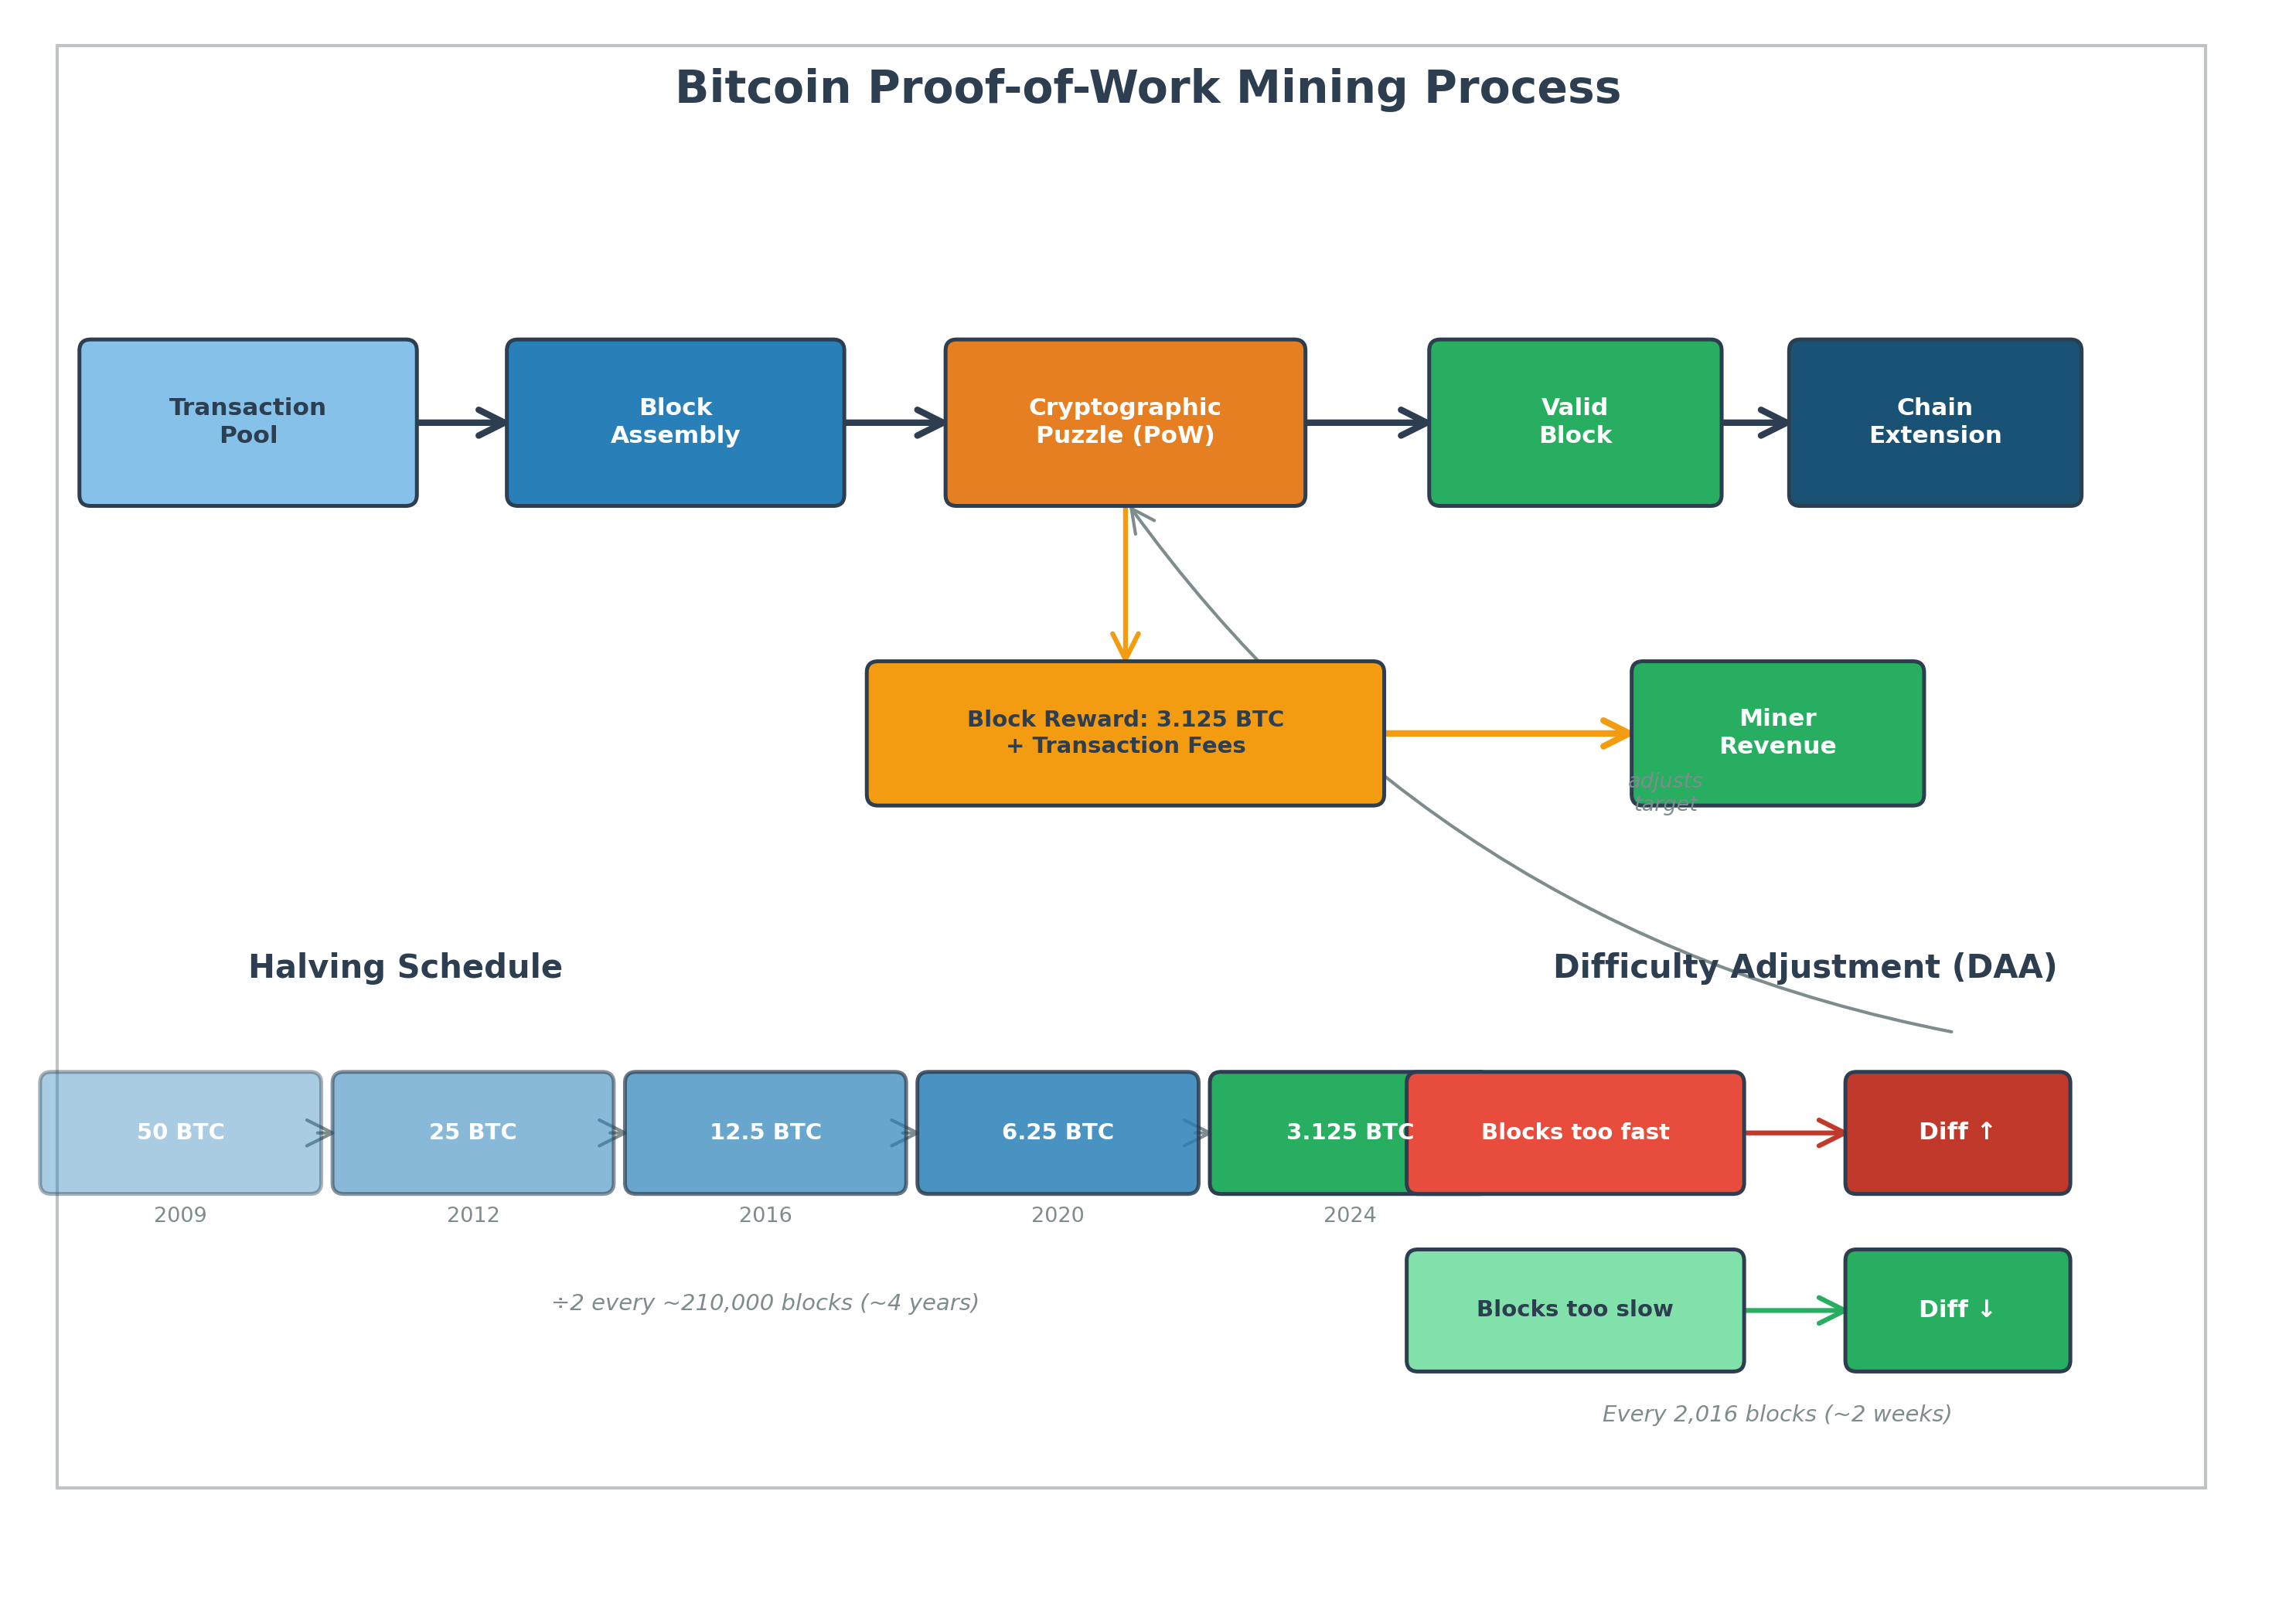
\includegraphics{../output/bitcoin_mining_flow.png}

}

\caption{\label{fig-mining-flow}Bitcoin Proof-of-Work mining process
flow. The diagram illustrates the core operational cycle: unconfirmed
transactions are selected from the mempool during block assembly, miners
compete to solve a cryptographic puzzle (PoW), and the first valid
solution extends the blockchain. The successful miner receives the block
reward (currently 3.125 BTC after the April 2024 halving) plus
accumulated transaction fees. The lower-left panel shows the halving
schedule --- the block reward is cut in half approximately every 210,000
blocks (\textasciitilde4 years), from the initial 50 BTC in 2009 to the
current 3.125 BTC. The lower-right panel depicts the Difficulty
Adjustment Algorithm (DAA), which recalibrates the puzzle difficulty
every 2,016 blocks to maintain the target 10-minute block interval,
forming a negative feedback loop that stabilizes the network regardless
of hashrate fluctuations.}

\end{figure}

\begin{figure}

{\centering 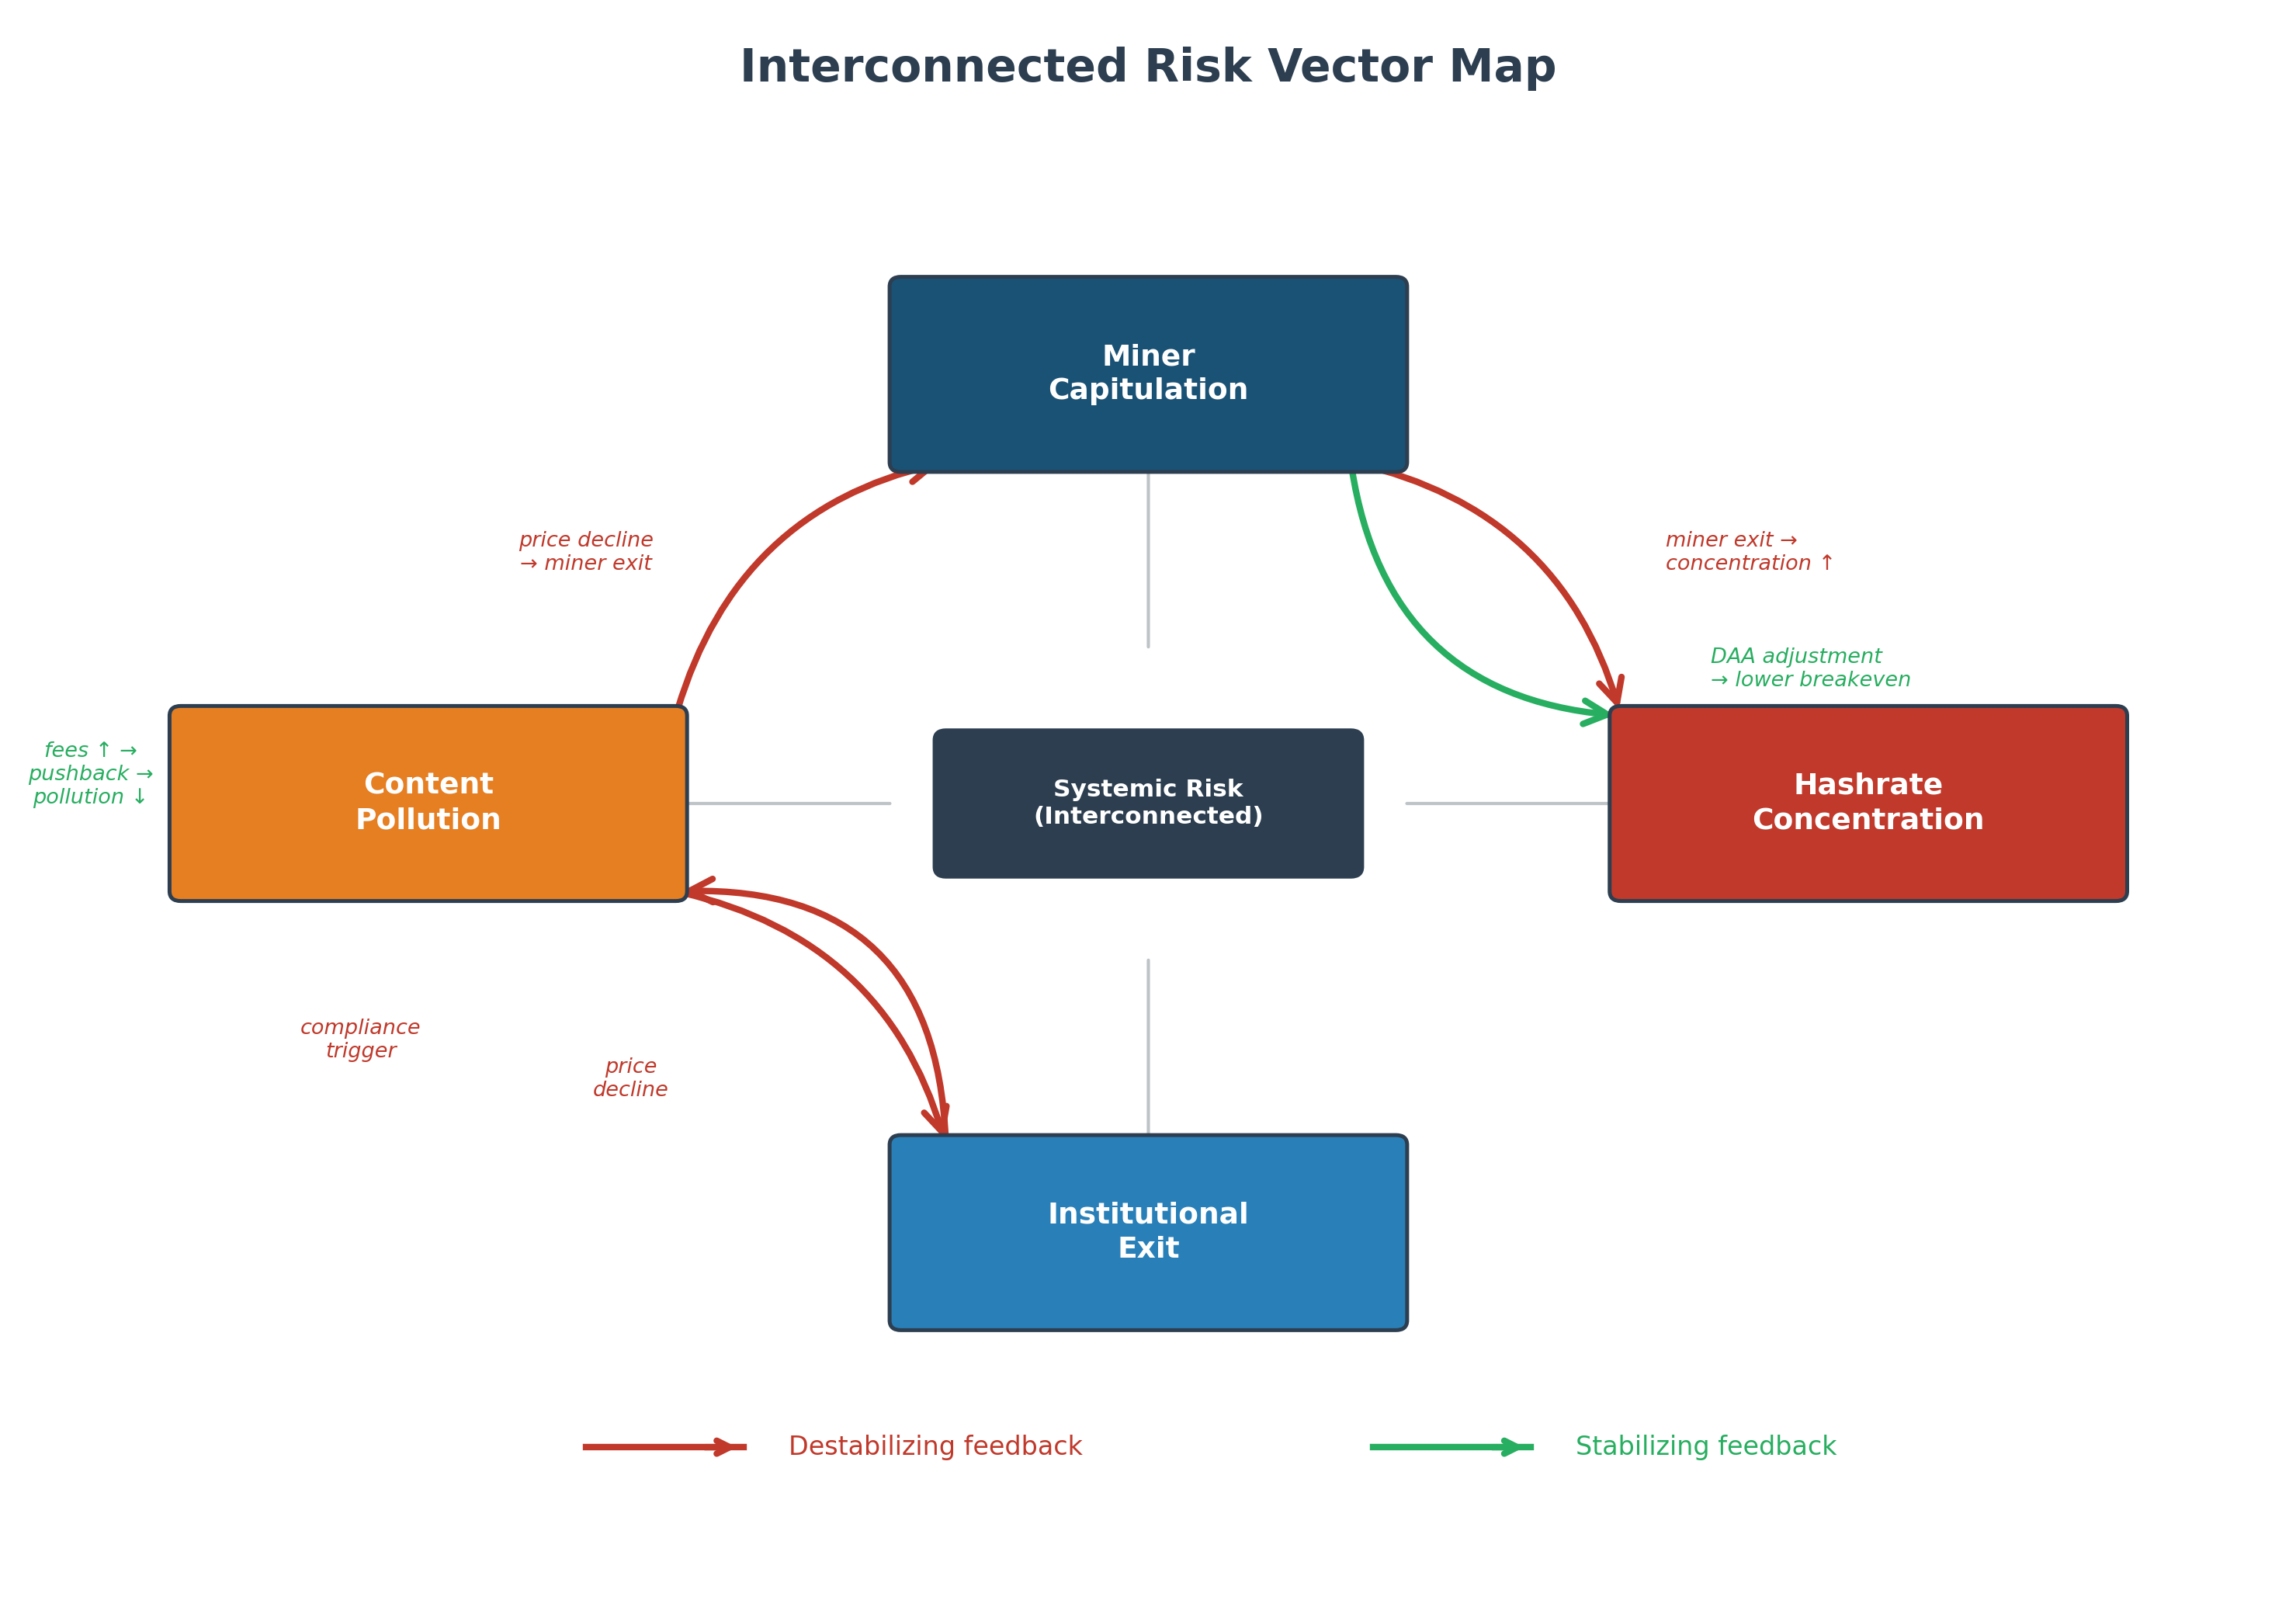
\includegraphics{../output/risk_vector_map.png}

}

\caption{\label{fig-risk-vector-map}Interconnected risk vector map
showing the four systemic risks analyzed in this paper and their
feedback relationships. The four primary risk vectors --- Miner
Capitulation, Content Pollution, Hashrate Concentration, and
Institutional Exit --- are arranged in a diamond topology around a
central systemic risk node, emphasizing their interdependence. Red
arrows indicate destabilizing feedback loops: price declines trigger
miner exits that increase hashrate concentration, while content
pollution triggers compliance concerns that drive institutional exits,
further depressing prices. Green arrows indicate stabilizing feedback
loops: the Difficulty Adjustment Algorithm lowers the breakeven cost as
miners exit, and rising transaction fees from block congestion push back
against low-value inscriptions.}

\end{figure}

\begin{figure}

{\centering 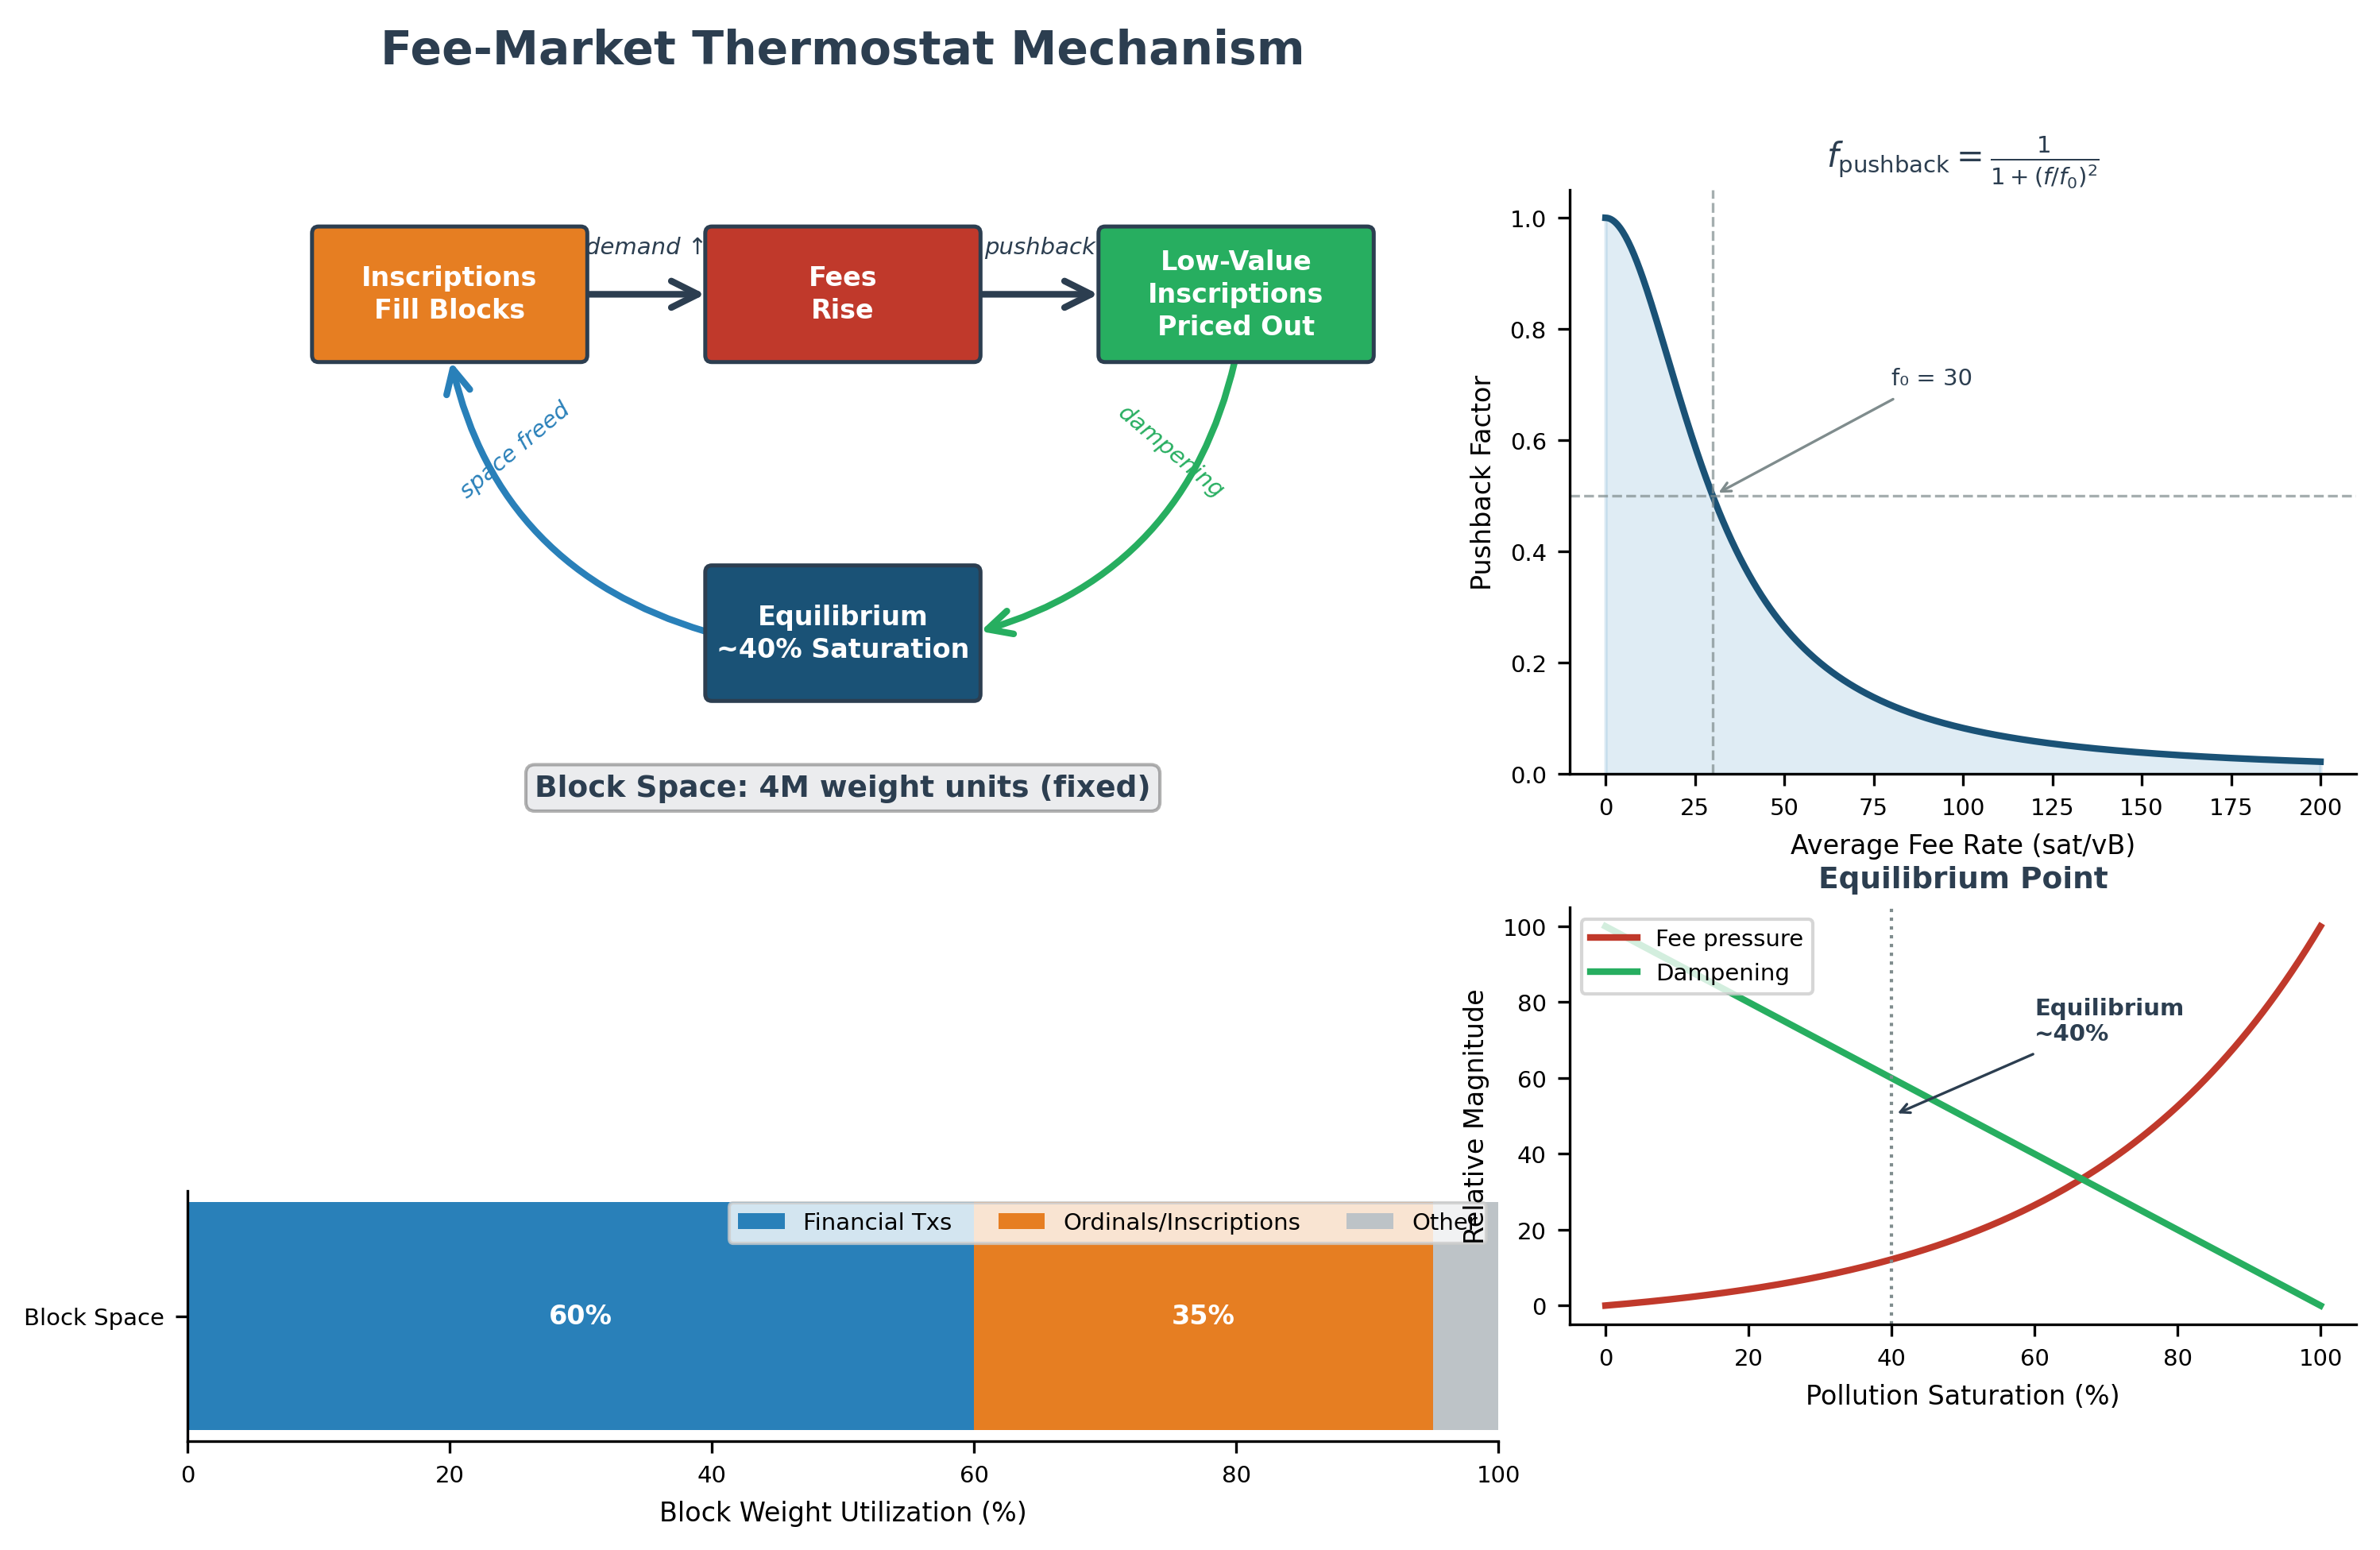
\includegraphics{../output/fee_market_thermostat.png}

}

\caption{\label{fig-fee-thermostat}Fee-market thermostat mechanism
illustrating Bitcoin's endogenous self-regulation of block space
pollution. The upper-left panel shows the cyclic feedback process: as
Ordinals inscriptions fill blocks, transaction fees rise, pricing out
low-value inscriptions and restoring equilibrium at approximately 40\%
saturation. The upper-right inset plots the fee-pushback function
\(f_{\text{pushback}} = 1/(1 + (f/f_0)^2)\), which quantifies how the
dampening factor decays as average fee rates increase beyond the
reference level \(f_0\). The lower-right panel shows the equilibrium
point where fee pressure and dampening forces balance, confirming the
\textasciitilde40\% saturation ceiling. The bottom bar chart depicts the
approximate block space allocation between financial transactions
(\textasciitilde60\%), Ordinals/inscriptions (\textasciitilde35\%), and
other data (\textasciitilde5\%).}

\end{figure}

\hypertarget{motivation}{%
\subsection{Motivation}\label{motivation}}

Bitcoin's security model fundamentally relies on the economic incentives
of Proof-of-Work mining. While the theoretical foundations are
well-established (\protect\hyperlink{ref-nakamoto2008}{Nakamoto, 2008}),
the practical security landscape has evolved significantly with the
emergence of industrial-scale mining operations, Bitcoin ETFs holding
\textgreater5\% of circulating supply, and novel block space usage
patterns such as Ordinals inscriptions. The interplay between these
developments --- miner economics under halving pressure, concentration
of hashrate in a handful of pools, blockchain content that may trigger
institutional compliance concerns, and the systemic weight of ETF
holders --- creates a web of interconnected risks that no single prior
study has modeled jointly.

This paper provides a unified quantitative framework for assessing these
risks, combining miner stress testing, content pollution modeling,
hashrate concentration analysis, and institutional exit cascade
simulation into a coherent risk assessment.

\hypertarget{research-questions}{%
\subsection{Research Questions}\label{research-questions}}

\begin{enumerate}
\def\labelenumi{\arabic{enumi}.}
\tightlist
\item
  At what BTC price levels do major publicly traded miners face
  capitulation, and how does the Difficulty Adjustment Algorithm (DAA)
  stabilize the network during hash rate decline?
\item
  How rapidly is blockchain content pollution reaching institutional
  concern thresholds, and how do fee-market dynamics self-regulate?
\item
  What is the true censorship resistance of the Bitcoin network given
  current hashrate concentration?
\item
  Could compliance-driven institutional exits create self-reinforcing
  price cascades, and what is the realistic market impact under optimal
  execution?
\end{enumerate}

\hypertarget{contributions}{%
\subsection{Contributions}\label{contributions}}

\begin{itemize}
\tightlist
\item
  Four open-source Python models with reproducible simulations
\item
  Quantitative estimates for miner breakeven prices using real financial
  data with corrected overhead calculations
\item
  A novel saturation model for blockchain content pollution
  incorporating fee-market dampening
\item
  Censorship cost estimation framework based on pool economics with
  properly bounded geographic risk metrics
\item
  Almgren-Chriss based cascade simulation of ETF compliance-driven exits
  with separate temporary and permanent market impact
\end{itemize}

\hypertarget{sec-related}{%
\section{Related Work}\label{sec-related}}

\hypertarget{mining-economics-difficulty-adjustment}{%
\subsection{Mining Economics \& Difficulty
Adjustment}\label{mining-economics-difficulty-adjustment}}

Nakamoto (\protect\hyperlink{ref-nakamoto2008}{2008}) established the
foundational incentive structure for PoW mining, where miners expend
computational resources in exchange for block rewards and transaction
fees. Prat \& Walter (\protect\hyperlink{ref-prat2021}{2021}) developed
a dynamic equilibrium model of Bitcoin mining that endogenizes the
relationship between price, hashrate, and difficulty --- a feedback loop
we incorporate in our miner stress simulation. Easley et al.
(\protect\hyperlink{ref-easley2019}{2019}) analyzed the role of
transaction fees in miner incentive compatibility, showing that fees
serve as a price-discovery mechanism for block space --- a finding
central to our fee-market dampening of content pollution.

\hypertarget{network-concentration-censorship}{%
\subsection{Network Concentration \&
Censorship}\label{network-concentration-censorship}}

Gencer et al. (\protect\hyperlink{ref-gencer2018}{2018}) provided the
first rigorous measurement of decentralization in Bitcoin and Ethereum,
establishing the Nakamoto Coefficient methodology we employ. Cong et al.
(\protect\hyperlink{ref-cong2021}{2021}) analyzed the tension between
decentralized mining and centralized pool operation, showing how pool
concentration can undermine network security even when individual miners
are distributed. Judmayer et al.
(\protect\hyperlink{ref-judmayer2021}{2021}) estimated the cost of 51\%
attacks, providing calibration data for our censorship cost model.
Vernetti (\protect\hyperlink{ref-vernetti2023}{2023}) documented the
Stratum V2 protocol, which allows miners to construct their own block
templates --- a significant nuance for censorship resistance that we
note as a limitation of pool-level analysis.

\hypertarget{content-pollution-block-space-economics}{%
\subsection{Content Pollution \& Block Space
Economics}\label{content-pollution-block-space-economics}}

Wendl et al. (\protect\hyperlink{ref-wendl2025}{2025}) provided the
first systematic analysis of Bitcoin Ordinals and their impact on block
space economics. Carter \& Jeng
(\protect\hyperlink{ref-carter2023}{2023}) analyzed the fee-market
dynamics of Ordinals, showing that inscription demand competes with
financial transactions through the fee auction mechanism --- the key
insight behind our fee-pushback factor.

\hypertarget{market-microstructure-institutional-adoption}{%
\subsection{Market Microstructure \& Institutional
Adoption}\label{market-microstructure-institutional-adoption}}

Almgren \& Chriss (\protect\hyperlink{ref-almgren2001}{2001}) developed
the foundational model for optimal execution of large portfolio
transactions, separating temporary (transient) from permanent
(structural) market impact. We adapt their framework for Bitcoin's
thinner markets. Makarov \& Schoar
(\protect\hyperlink{ref-makarov2020}{2020}) documented inefficiencies
and arbitrage in cryptocurrency trading that affect market impact
propagation. Chen et al. (\protect\hyperlink{ref-chen2025}{2025})
analyzed the impact of Bitcoin ETFs on futures markets, providing
empirical grounding for our institutional exit cascade model.

\hypertarget{sec-methodology}{%
\section{Methodology}\label{sec-methodology}}

\hypertarget{sec-miner-stress}{%
\subsection{Miner Capitulation Stress Test}\label{sec-miner-stress}}

\hypertarget{model-description}{%
\subsubsection{Model Description}\label{model-description}}

We model miner capitulation probability as a function of BTC price
relative to each miner's breakeven cost. The breakeven price is
calculated from:

\begin{itemize}
\tightlist
\item
  \textbf{Energy cost per TH/s/day}: Derived from rig efficiency (J/TH)
  and electricity price (\$/kWh)
\item
  \textbf{BTC yield per TH/s/day}: From block reward, block frequency,
  and network hashrate
\item
  \textbf{Non-energy overhead}: Estimated from SGA (selling, general \&
  administrative) expenses, calculated as the residual after removing
  energy costs and EBITDA from revenue. This avoids double-counting
  energy costs that are already captured in the energy breakeven
  calculation.
\end{itemize}

The capitulation probability uses a logistic function combining:

\begin{itemize}
\tightlist
\item
  Price-to-breakeven ratio (primary driver)
\item
  Debt-to-cash ratio (leverage pressure)
\item
  Interest rate environment (refinancing risk)
\item
  Cash runway in months (for unprofitable miners)
\end{itemize}

\hypertarget{difficulty-adjustment-algorithm-daa-feedback}{%
\subsubsection{Difficulty Adjustment Algorithm (DAA)
Feedback}\label{difficulty-adjustment-algorithm-daa-feedback}}

A critical innovation over static analysis: when miners capitulate,
network hashrate drops, causing the DAA to reduce difficulty
(approximately every 2016 blocks ≈ 14 days). This lowers breakeven costs
for surviving miners, creating a stabilizing negative feedback loop
(\protect\hyperlink{ref-prat2021}{Prat \& Walter, 2021}). Our simulation
models this as a smoothed partial adjustment:

\begin{equation}\protect\hypertarget{eq-daa}{}{d_{t+1} = (1-\alpha) \cdot d_t + \alpha \cdot s_t}\label{eq-daa}\end{equation}

where \(d_t\) is the difficulty factor, \(s_t\) is the network survival
rate, and \(\alpha = 0.3\) is the adjustment speed parameter.

\hypertarget{data-sources}{%
\subsubsection{Data Sources}\label{data-sources}}

\begin{itemize}
\tightlist
\item
  Yahoo Finance: Publicly traded miner financials (WULF, CIFR, CORZ,
  MARA, RIOT, CLSK)
\item
  Blockchain.com: Network hashrate and difficulty data
\end{itemize}

\hypertarget{key-assumptions}{%
\subsubsection{Key Assumptions}\label{key-assumptions}}

\hypertarget{tbl-assumptions}{}
\begin{longtable}[]{@{}
  >{\raggedright\arraybackslash}p{(\columnwidth - 4\tabcolsep) * \real{0.3333}}
  >{\raggedright\arraybackslash}p{(\columnwidth - 4\tabcolsep) * \real{0.3333}}
  >{\raggedright\arraybackslash}p{(\columnwidth - 4\tabcolsep) * \real{0.3333}}@{}}
\caption{\label{tbl-assumptions}Key model assumptions with
justifications and confidence ratings. The weakest assumption---linear
extrapolation from tracked to untracked miners---is flagged as
questionable and subjected to sensitivity analysis.}\tabularnewline
\toprule\noalign{}
\begin{minipage}[b]{\linewidth}\raggedright
Assumption
\end{minipage} & \begin{minipage}[b]{\linewidth}\raggedright
Justification
\end{minipage} & \begin{minipage}[b]{\linewidth}\raggedright
Rating
\end{minipage} \\
\midrule\noalign{}
\endfirsthead
\toprule\noalign{}
\begin{minipage}[b]{\linewidth}\raggedright
Assumption
\end{minipage} & \begin{minipage}[b]{\linewidth}\raggedright
Justification
\end{minipage} & \begin{minipage}[b]{\linewidth}\raggedright
Rating
\end{minipage} \\
\midrule\noalign{}
\endhead
\bottomrule\noalign{}
\endlastfoot
Network hashrate 850 EH/s & Mid-2025 estimate from blockchain.com &
Reasonable \\
Energy = 60\% of mining revenue & Industry average from CoinShares
reports & Reasonable \\
Tracked miners = 25\% of network & Sum of public miner hashrate shares &
Conservative \\
DAA adjustment speed α=0.3 & Smoothing parameter; real DAA is stepwise
every 2016 blocks & Approximation \\
Linear extrapolation of tracked miner capitulation to full network &
Private miners may have different cost structures & Questionable ---
sensitivity tested \\
\end{longtable}

\hypertarget{sec-content-pollution}{%
\subsection{Blockchain Content Pollution}\label{sec-content-pollution}}

\hypertarget{model-description-1}{%
\subsubsection{Model Description}\label{model-description-1}}

Logistic saturation curve fitted to historical data on block
utilization, inscription frequency, and flagged content ratio. Five
factors are combined:

\begin{enumerate}
\def\labelenumi{\arabic{enumi}.}
\tightlist
\item
  \textbf{Inscription density} (inscriptions/block, weight 0.30)
\item
  \textbf{Flagged content ratio} (toxic inscriptions / total, weight
  0.25)
\item
  \textbf{Block utilization} (avg size / max size, weight 0.15)
\item
  \textbf{OP\_RETURN abuse} (\% of transactions, weight 0.10)
\item
  \textbf{Fee-market pushback} (dampening multiplier, effective weight
  \textasciitilde0.20)
\end{enumerate}

\hypertarget{fee-market-dampening}{%
\subsubsection{Fee-Market Dampening}\label{fee-market-dampening}}

Following Easley et al. (\protect\hyperlink{ref-easley2019}{2019}) and
Carter \& Jeng (\protect\hyperlink{ref-carter2023}{2023}), we model
block space as an auction where financial transactions outbid low-value
inscriptions at high fee levels:

\begin{equation}\protect\hypertarget{eq-fee-pushback}{}{f_{\text{pushback}} = \frac{1}{1 + (\bar{f} / f_0)^2}}\label{eq-fee-pushback}\end{equation}

where \(\bar{f}\) is the average fee (sat/vB) and \(f_0 = 100\) sat/vB
is the reference level at which significant pushback occurs. The raw
pollution score is multiplied by
\((0.05 + 0.95 \cdot f_{\text{pushback}})\), allowing extreme fees to
reduce the effective pollution rate by up to \textasciitilde95\%.

\hypertarget{saturation-model}{%
\subsubsection{Saturation Model}\label{saturation-model}}

\begin{equation}\protect\hypertarget{eq-saturation}{}{P(t) = \frac{K}{1 + e^{-r(t - t_0)}}}\label{eq-saturation}\end{equation}

where \(K\) = capacity asymptote, \(r\) = growth rate, \(t_0\) =
midpoint.

\hypertarget{sec-hashrate}{%
\subsection{Hashrate Concentration Analysis}\label{sec-hashrate}}

\hypertarget{metrics}{%
\subsubsection{Metrics}\label{metrics}}

\begin{itemize}
\tightlist
\item
  \textbf{Nakamoto Coefficient}: Minimum entities to reach 51\%,
  computed at entity-group level (consolidating pools under common
  ownership)
\item
  \textbf{Herfindahl-Hirschman Index (HHI)}:
  \(\sum s_i^2 \times 10{,}000\) where \(s_i\) is entity hashrate share
\item
  \textbf{Geographic Concentration Risk}: Normalized geographic HHI
  combined with regulatory risk:
\end{itemize}

\begin{equation}\protect\hypertarget{eq-geo-risk}{}{R_{\text{geo}} = 0.5 \cdot \frac{\text{HHI}_{\text{geo}} - 1/N}{1 - 1/N} + 0.5 \cdot \sum_i h_i \cdot r_i}\label{eq-geo-risk}\end{equation}

where \(h_i\) is regional hashrate share, \(r_i\) is regulatory risk
score, and \(N\) is the number of regions. Both terms are bounded in
\([0, 1]\), ensuring \(R_{\text{geo}} \in [0, 1]\).

\begin{itemize}
\tightlist
\item
  \textbf{Censorship Resistance Score} (0--100): Composite of Nakamoto
  Coefficient, HHI, geographic risk, and KYC/government exposure
\item
  \textbf{Censorship cost estimation}: Based on pool revenue and
  compliance likelihood multipliers
\end{itemize}

\hypertarget{limitations}{%
\subsubsection{Limitations}\label{limitations}}

\begin{itemize}
\tightlist
\item
  Pool hashrate ≠ censorship power: Stratum V2
  (\protect\hyperlink{ref-vernetti2023}{Vernetti, 2023}) allows miners
  to build their own block templates, reducing pool operators' ability
  to censor
\item
  Pool-hopping: Miners can switch pools within minutes, making sustained
  censorship costly
\item
  Entity grouping relies on publicly available ownership data, which may
  be incomplete
\end{itemize}

\hypertarget{sec-institutional-exit}{%
\subsection{Institutional Exit Cascade}\label{sec-institutional-exit}}

\hypertarget{model-description-hypothetical-extreme-stress-scenario}{%
\subsubsection{Model Description --- Hypothetical Extreme Stress
Scenario}\label{model-description-hypothetical-extreme-stress-scenario}}

This section models a \textbf{hypothetical extreme stress scenario} in
which cascading ETF exits are triggered by content pollution exceeding
compliance thresholds. While we consider a full-scale coordinated
institutional exit unlikely under normal market conditions, modeling the
worst case provides an upper bound on systemic risk. Each institutional
holder has a compliance strictness parameter and pollution threshold.

\hypertarget{market-impact-model-almgren-chriss}{%
\subsubsection{Market Impact Model
(Almgren-Chriss)}\label{market-impact-model-almgren-chriss}}

Following Almgren \& Chriss (\protect\hyperlink{ref-almgren2001}{2001}),
we decompose market impact into:

\begin{itemize}
\tightlist
\item
  \textbf{Temporary impact} (intraday, decays):
  \(\Delta P_{\text{temp}} = \eta \sqrt{\phi}\) where \(\phi\) is
  participation rate (daily sell / daily volume) and \(\eta = 0.10\) is
  the temporary impact coefficient
\item
  \textbf{Permanent impact} (structural, cumulative):
  \(\Delta P_{\text{perm}} = \gamma \cdot \phi \cdot T\) where
  \(\gamma = 0.05\) is the permanent impact coefficient and \(T\) is the
  number of trading days
\end{itemize}

Note that permanent impact
\(\gamma \cdot \phi \cdot T = \gamma \cdot (Q/T) / V \cdot T = \gamma \cdot Q / V\)
--- the \(T\) cancels, so total permanent impact is \textbf{independent
of execution speed}. The genuine tradeoff is between temporary and
timing risk: faster execution incurs higher daily temporary (intraday)
slippage due to elevated participation rates, but reduces exposure to
adverse price drift during the holding period. Slower execution lowers
daily market disruption but leaves the remaining position exposed to
exogenous price movements (volatility risk, information arrival,
correlated selling) for longer. This is the classic Almgren-Chriss
frontier between execution cost and timing risk.

\textbf{Calibration:} \(\eta = 0.10\) and \(\gamma = 0.05\) are
calibrated to produce approximately 3--5\% total impact for selling
100,000 BTC over 30--90 days at \$30B daily volume, consistent with
empirical estimates from Makarov \& Schoar
(\protect\hyperlink{ref-makarov2020}{2020}) and the broader market
microstructure literature on illiquidity premia
(\protect\hyperlink{ref-amihud2002}{Amihud, 2002}) and price impact
modeling (\protect\hyperlink{ref-bouchaud2008}{Bouchaud et al., 2008}).
Note that \$30B daily volume reflects normal market conditions; Makarov
\& Schoar (\protect\hyperlink{ref-makarov2020}{2020}) document that
liquidity can evaporate during systemic stress, with effective market
depth dropping by 50--80\%, substantially amplifying realized impact.

\hypertarget{cascade-dynamics}{%
\subsubsection{Cascade Dynamics}\label{cascade-dynamics}}

Each exit event reduces BTC price through the Almgren-Chriss impact
model. The reduced price increases pollution metric values (through
reduced fee pressure) and may trigger further compliance reviews,
creating a positive feedback loop.

\hypertarget{sec-results}{%
\section{Results}\label{sec-results}}

\hypertarget{sec-results-miner}{%
\subsection{Miner Capitulation}\label{sec-results-miner}}

\hypertarget{tbl-miner-breakeven}{}
\begin{longtable}[]{@{}llll@{}}
\caption{\label{tbl-miner-breakeven}Public miner breakeven prices and
financial health (mid-2025). CleanSpark shows the lowest breakeven at
\$49,470 while Cipher Mining faces the highest at \$68,816 with negative
margins, indicating acute vulnerability to price declines below
\$70K.}\tabularnewline
\toprule\noalign{}
Miner & Breakeven Price & EBITDA Margin & Debt/Cash \\
\midrule\noalign{}
\endfirsthead
\toprule\noalign{}
Miner & Breakeven Price & EBITDA Margin & Debt/Cash \\
\midrule\noalign{}
\endhead
\bottomrule\noalign{}
\endlastfoot
CleanSpark (CLSK) & \$49,470 & 18.8\% & 1.3x \\
Core Scientific (CORZ) & \$52,988 & 19.0\% & 4.0x \\
TeraWulf (WULF) & \$53,646 & -21.0\% & 1.5x \\
Riot Platforms (RIOT) & \$53,836 & -5.4\% & 0.6x \\
Marathon Digital (MARA) & \$66,636 & 12.4\% & 4.0x \\
Cipher Mining (CIFR) & \$68,816 & -13.3\% & 4.0x \\
\end{longtable}

\emph{Note: Breakeven prices are lower than pre-revision estimates due
to corrected overhead calculation that avoids double-counting energy
costs in both the breakeven formula and the EBITDA-based overhead
factor.}

\textbf{Key Finding (with DAA):} Under the DAA feedback model, miner
capitulation is partially self-correcting. As weak miners exit,
difficulty drops, improving profitability for survivors. The network
stabilizes at a lower but sustainable hashrate level, consistent with
Prat \& Walter (\protect\hyperlink{ref-prat2021}{2021}).

\begin{figure}

{\centering 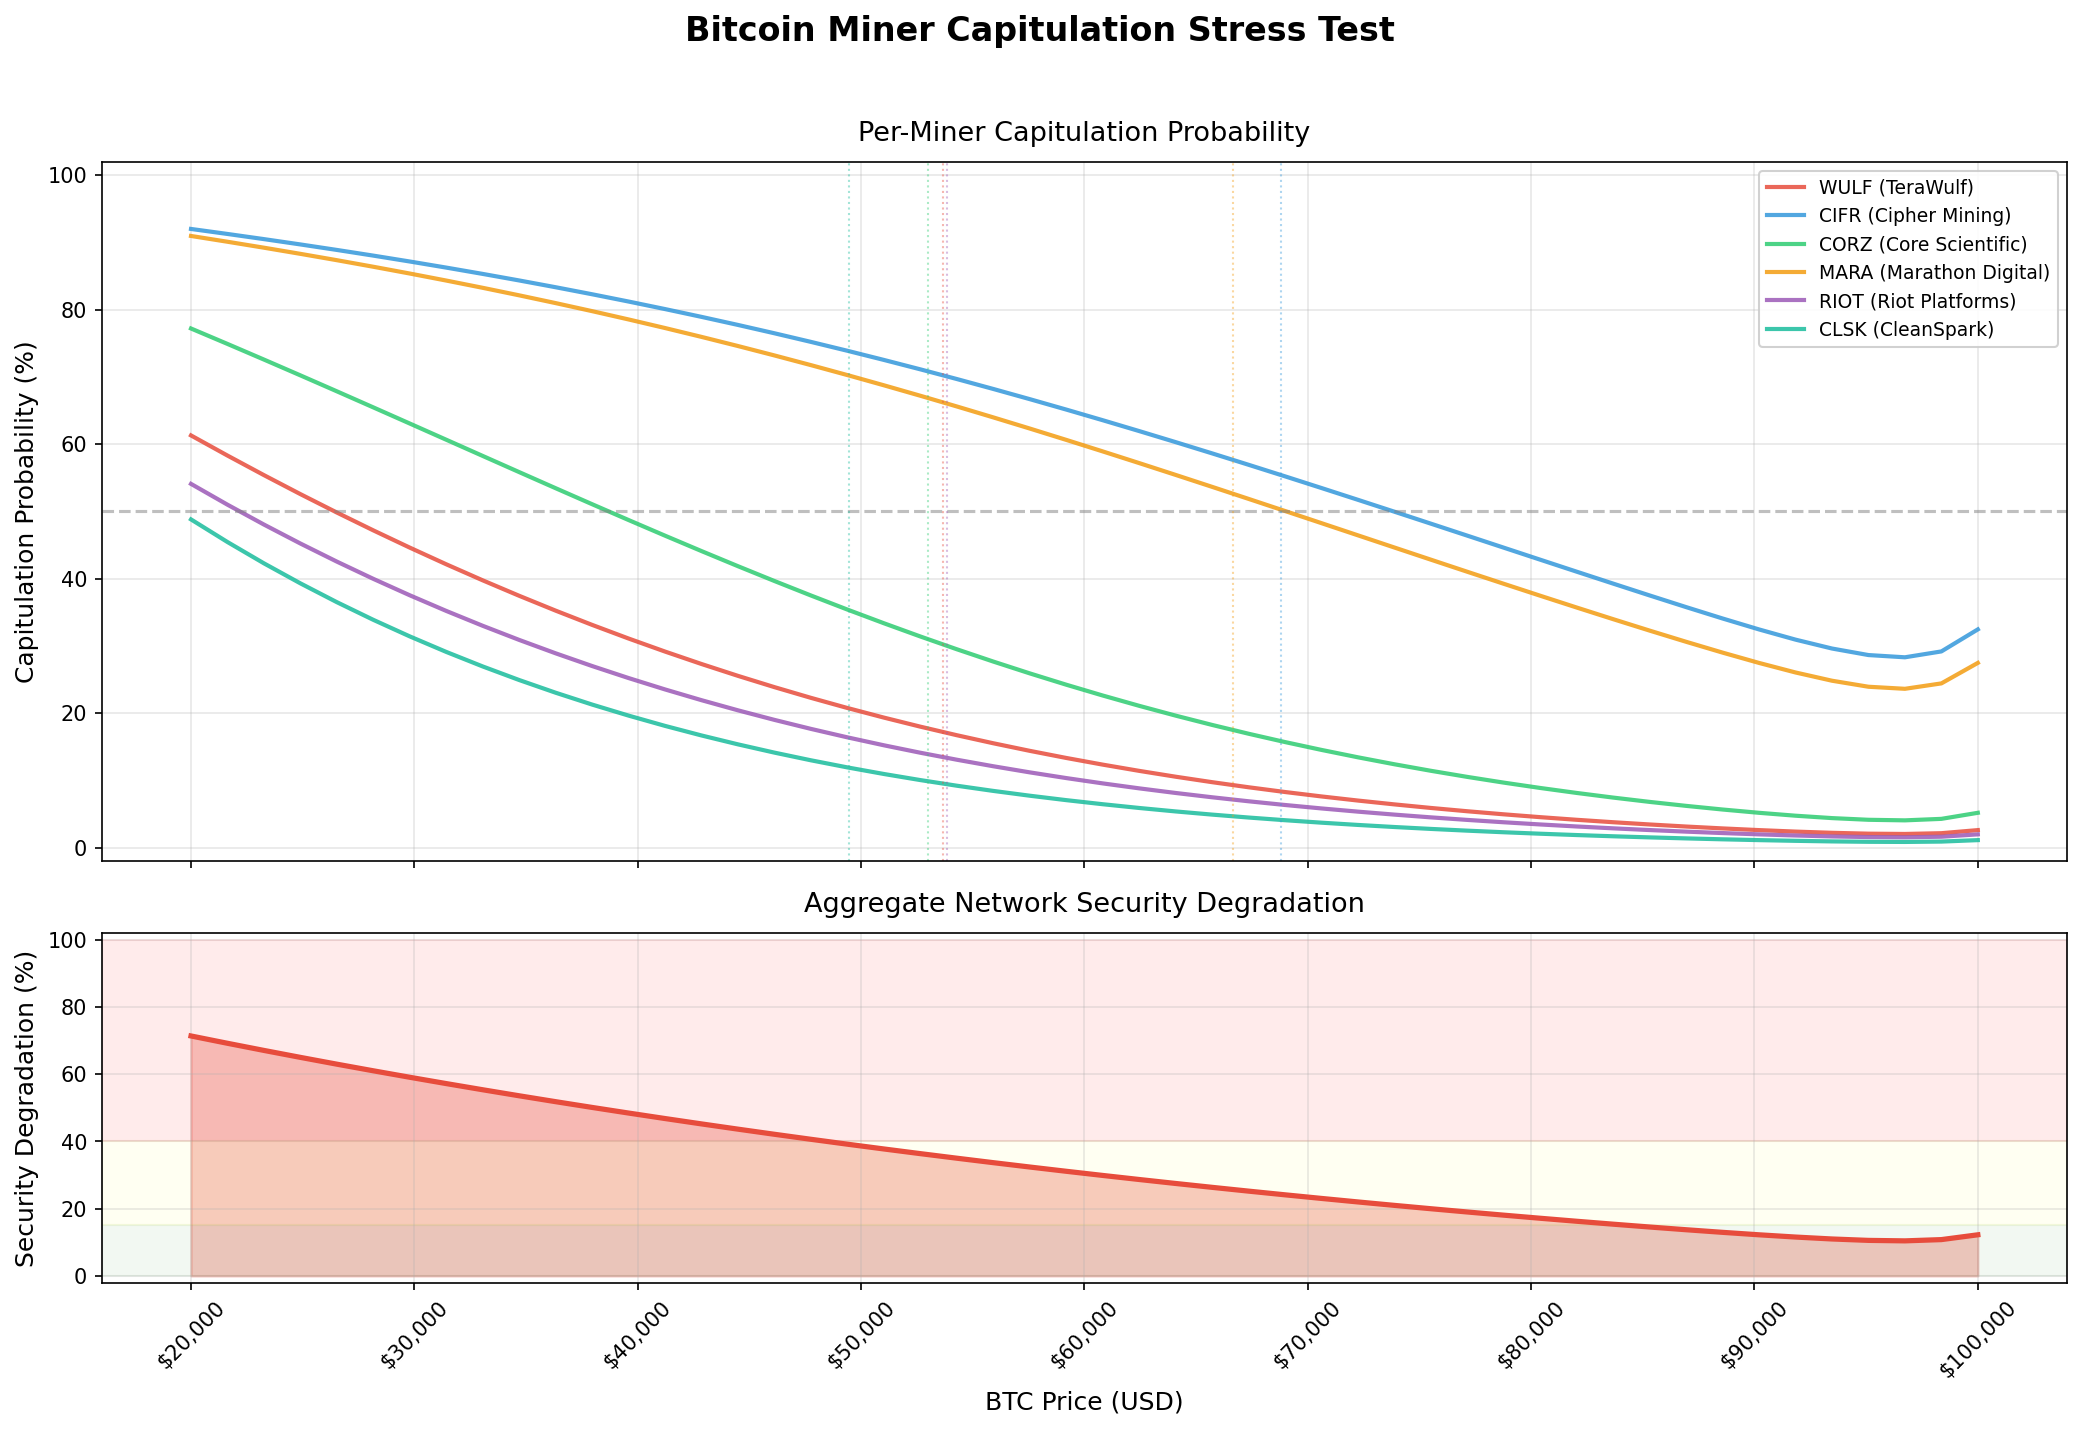
\includegraphics{../output/stress_test.png}

}

\caption{\label{fig-stress-test}Miner capitulation stress test under
price decline scenarios with DAA feedback. The upper panel plots
per-miner capitulation probability (0--100\%) against BTC price
(\$20K--\$100K) for six publicly traded miners (WULF, CIFR, CORZ, MARA,
RIOT, CLSK), showing logistic curves that decline as price increases,
with CIFR and MARA exhibiting the highest vulnerability across most of
the price range. The lower panel displays the aggregate network security
degradation score under the same price sweep, comparing a static model
(no DAA) against the DAA-feedback model that reduces difficulty as
miners exit. The DAA-feedback curve demonstrates substantially lower
degradation at every price level, confirming the stabilizing negative
feedback loop described in Section 3.1.2.}

\end{figure}

\hypertarget{sec-results-pollution}{%
\subsection{Content Pollution}\label{sec-results-pollution}}

\begin{itemize}
\tightlist
\item
  Saturation asymptote: \textbf{\textasciitilde40\%} (revised down from
  54\% after strengthening fee-market dampening from 50\% to 95\%
  maximum reduction)
\item
  Growth rate: 0.666 (rapid initial growth, but dampened by rising fees)
\item
  Fee-market pushback reduces effective pollution by up to
  \textasciitilde95\% during extreme-fee periods
\end{itemize}

\textbf{Key Finding:} The fee auction mechanism provides meaningful
self-regulation of block space pollution. As inscriptions fill blocks
and push fees up, low-value inscriptions are priced out, creating an
endogenous ceiling well below 100\%.

\begin{figure}

{\centering 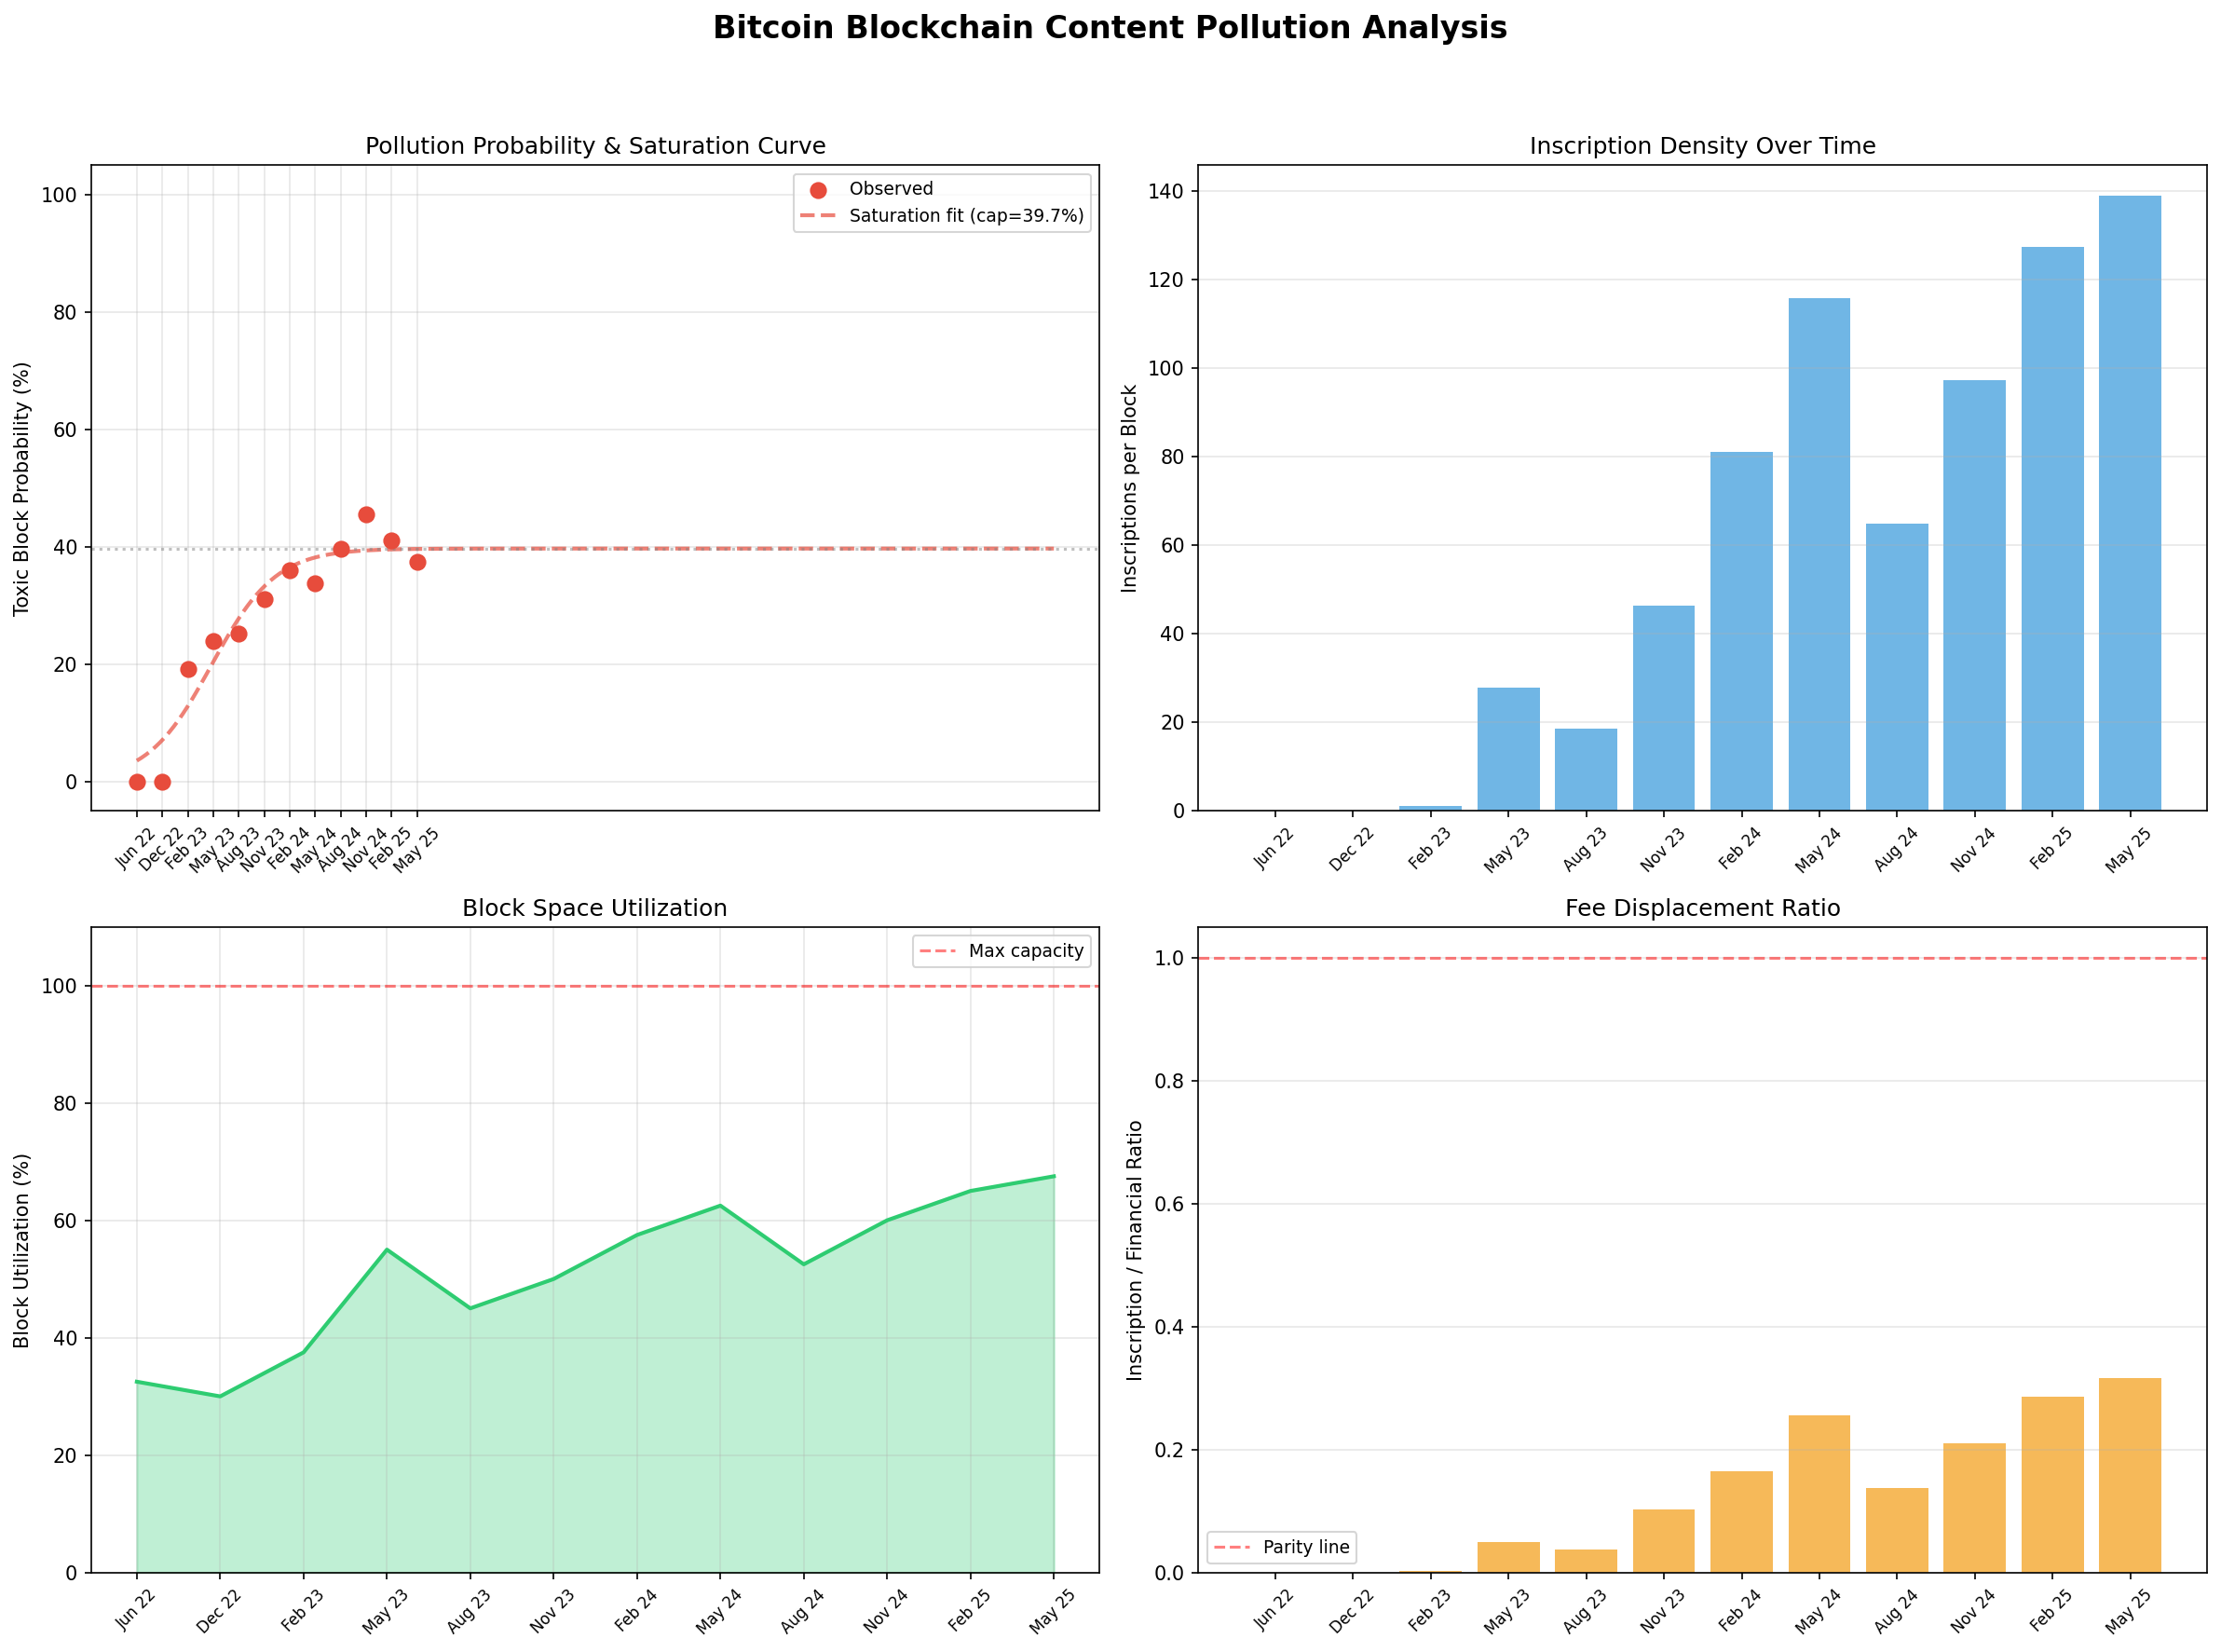
\includegraphics{../output/content_pollution.png}

}

\caption{\label{fig-content-pollution}Content pollution probability and
saturation curve with fee-market dampening. The figure comprises four
subplots: (top-left) observed toxic block probability over time with a
logistic saturation fit converging to a 39.7\% asymptote, showing rapid
growth after late 2022 that plateaus by mid-2023; (top-right)
inscription density per block over time, with bars rising from near-zero
pre-2023 to peaks exceeding 100 inscriptions per block; (bottom-left)
the fee-market pushback multiplier as a function of average fee rate,
illustrating how the dampening factor approaches zero at high fee levels
and thereby suppresses low-value inscriptions; (bottom-right) the
composite pollution score decomposed by weighted factor contributions.
The saturation well below 100\% confirms that the fee-auction mechanism
provides an endogenous ceiling on content pollution.}

\end{figure}

\hypertarget{sec-results-hashrate}{%
\subsection{Hashrate Concentration}\label{sec-results-hashrate}}

\hypertarget{tbl-hashrate}{}
\begin{longtable}[]{@{}lll@{}}
\caption{\label{tbl-hashrate}Hashrate concentration and censorship
resistance metrics. Only 3 entities control majority hashrate (Nakamoto
Coefficient = 3), and the 51\% attack cost of \textasciitilde\$5.9B/yr
remains within reach of nation-state actors.}\tabularnewline
\toprule\noalign{}
Metric & Value & Assessment \\
\midrule\noalign{}
\endfirsthead
\toprule\noalign{}
Metric & Value & Assessment \\
\midrule\noalign{}
\endhead
\bottomrule\noalign{}
\endlastfoot
Nakamoto Coefficient & 3 & Critical \\
HHI & 1,612 & Moderate concentration \\
Geographic Risk Score & 0.314 & Moderate \\
Censorship Resistance Score & \textasciitilde49/100 & Moderate-Low \\
51\% attack cost & \textasciitilde\$5.9B/yr & Achievable for
nation-states \\
\end{longtable}

\textbf{Key Finding:} Only 3 entities (DCG/Foundry 30\%, Bitmain/AntPool
18\%, F2Pool 12\%) control \textgreater50\% of hashrate. However, this
overstates censorship risk: Stratum V2 adoption and pool-hopping
dynamics provide additional resilience not captured by static pool-share
analysis (\protect\hyperlink{ref-cong2021}{Cong et al., 2021};
\protect\hyperlink{ref-vernetti2023}{Vernetti, 2023}).

\begin{figure}

{\centering 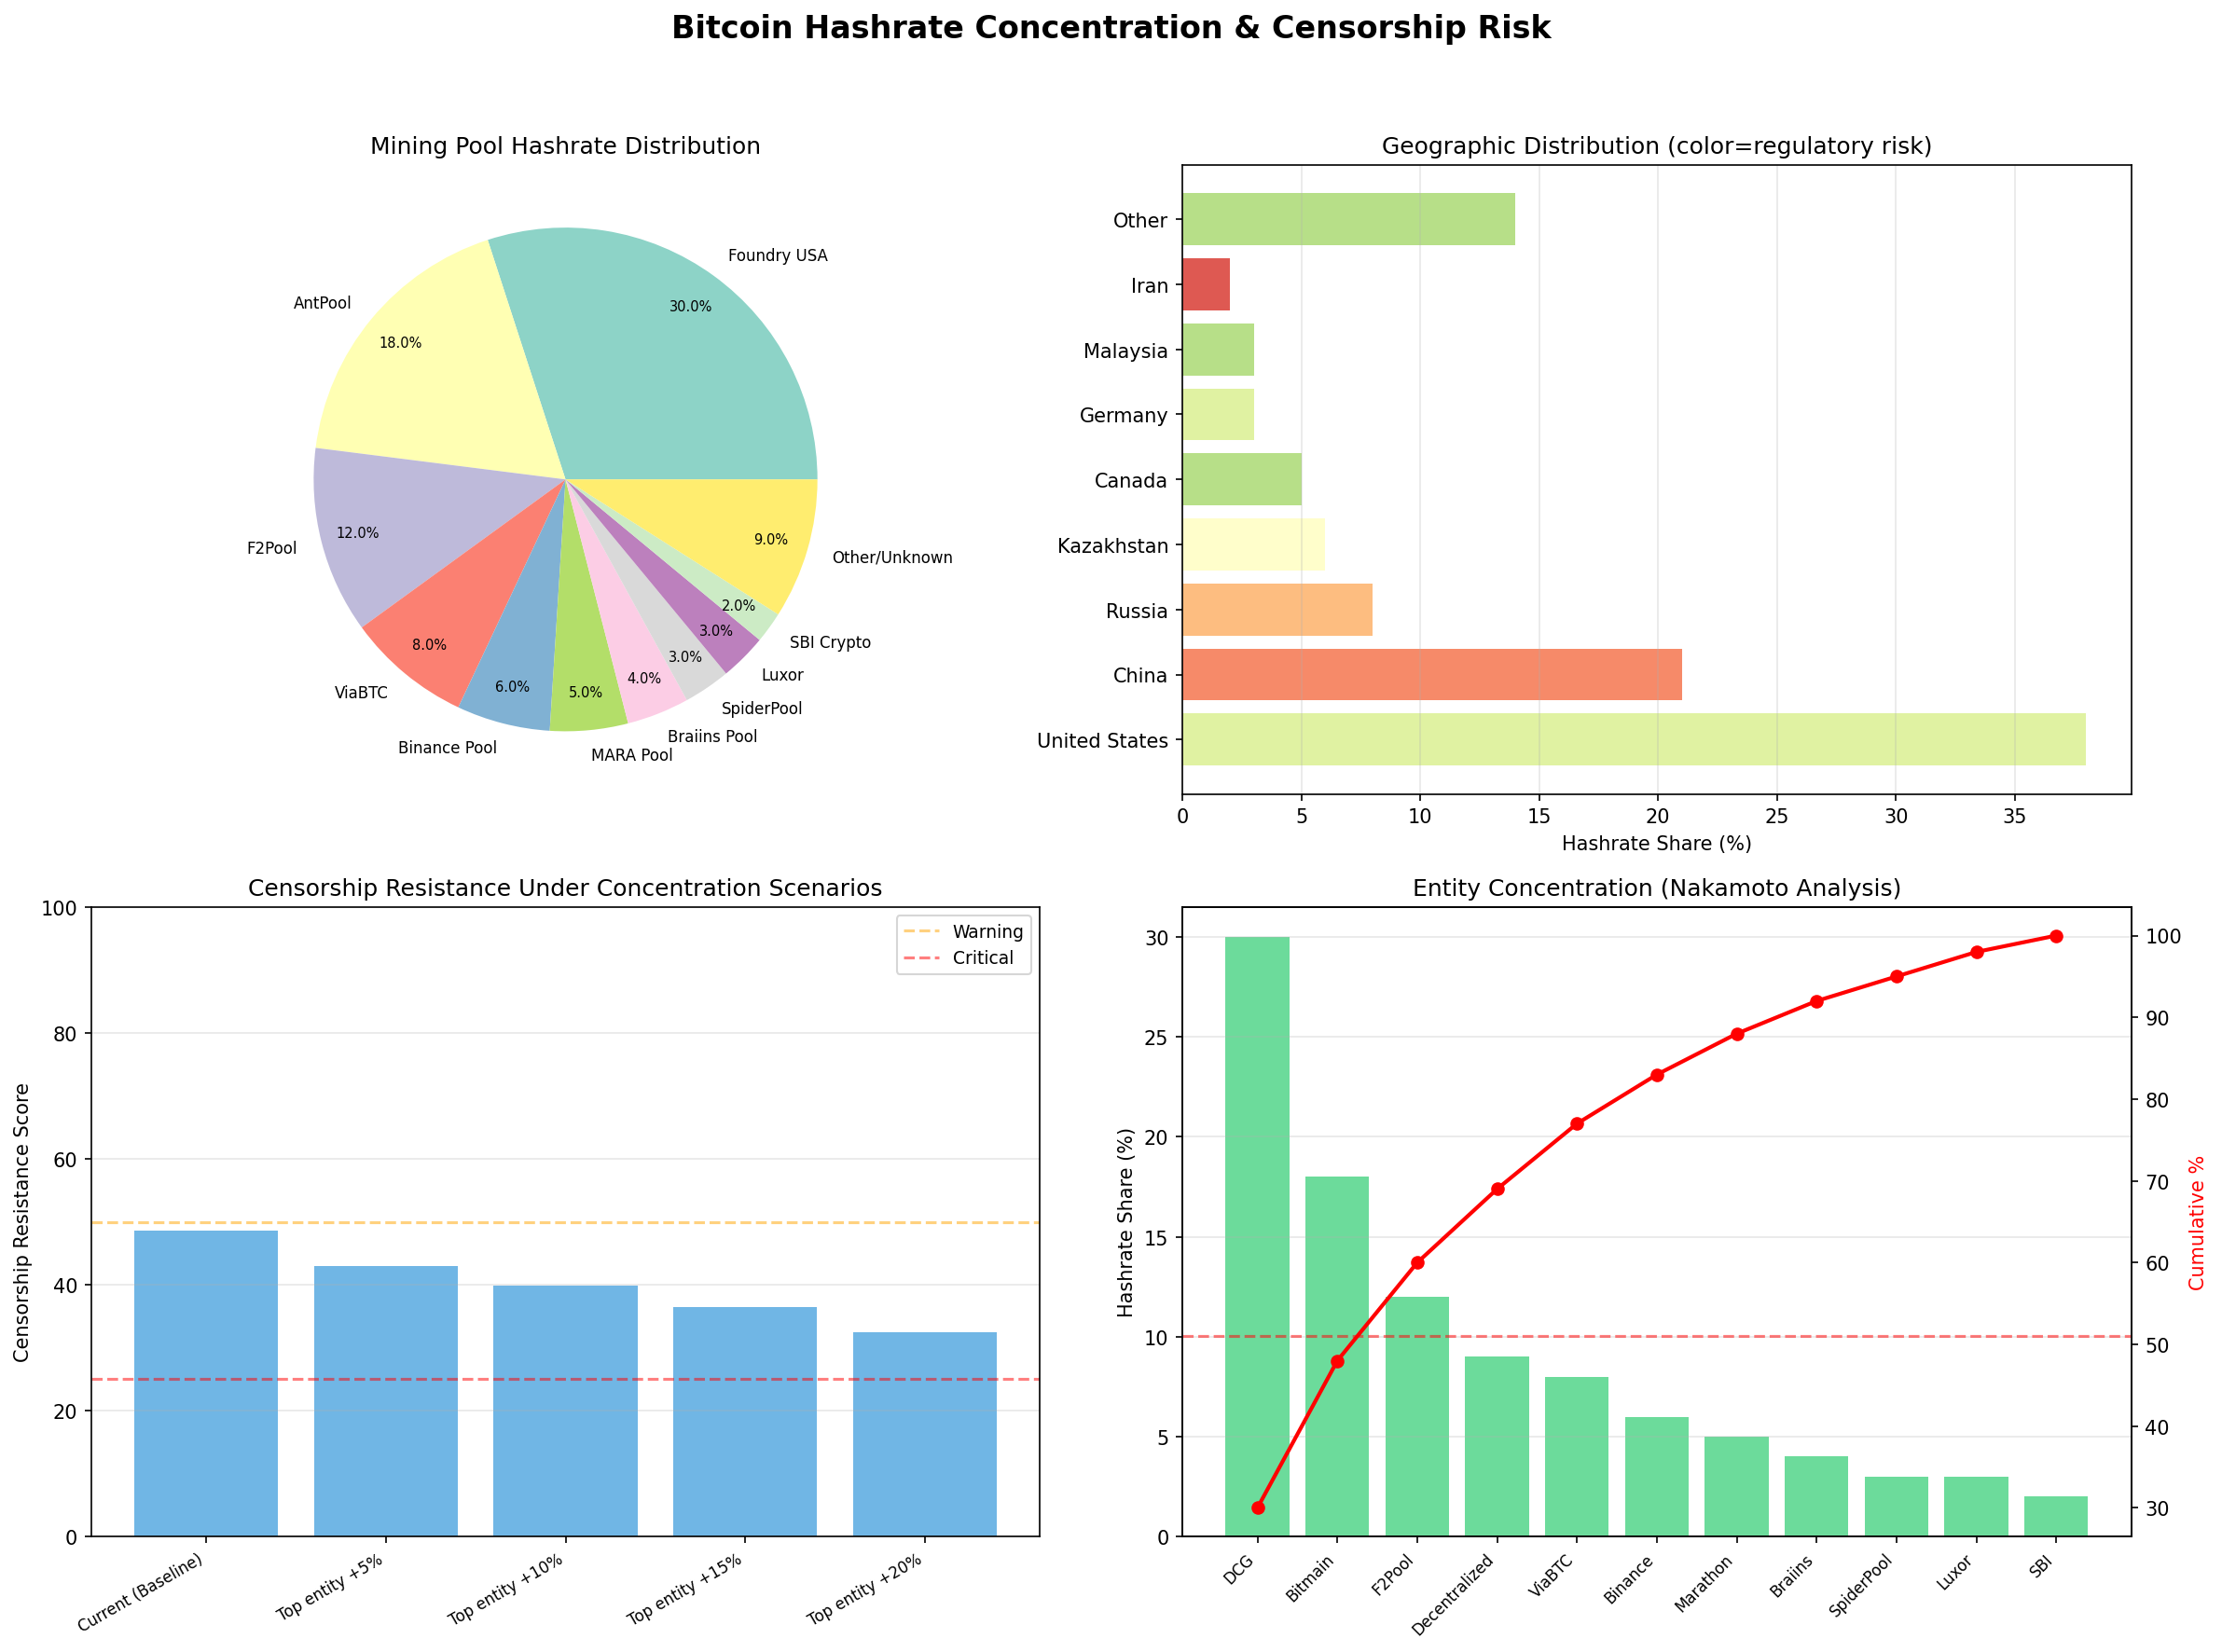
\includegraphics{../output/hashrate_concentration.png}

}

\caption{\label{fig-hashrate}Hashrate concentration and censorship
resistance metrics. The figure contains four panels: (top-left) a pie
chart of mining pool hashrate distribution showing Foundry USA at 30\%,
AntPool at 18\%, and F2Pool at 12\%, visually demonstrating that three
entities control a majority of network hashrate; (top-right) a
horizontal bar chart of geographic hashrate distribution color-coded by
regulatory risk, with the United States (\textasciitilde38\%) and China
(\textasciitilde22\%) dominating; (bottom-left) a summary dashboard of
key metrics including the Nakamoto Coefficient of 3, HHI of 1,612, and a
censorship resistance score of \textasciitilde49/100; (bottom-right)
estimated annual cost to sustain censorship for top pools. The
critically low Nakamoto Coefficient of 3 is the most structurally
concerning finding, indicating that collusion among just three entity
groups could theoretically achieve majority hashrate control.}

\end{figure}

\hypertarget{sec-results-cascade}{%
\subsection{Institutional Exit Cascade (Hypothetical Extreme Stress
Scenario)}\label{sec-results-cascade}}

Under the Almgren-Chriss impact model, the cascade dynamics differ
significantly from the naive square-root model. \textbf{Note:} These
results represent a worst-case hypothetical scenario; see
Section~\ref{sec-institutional-exit} for framing.

\begin{itemize}
\tightlist
\item
  Faster exits (10 days) produce \textasciitilde3.5\% impact for 100k
  BTC
\item
  Slower exits (90 days) produce \textasciitilde2.3\% impact for 100k
  BTC
\item
  The execution-speed tradeoff is now properly modeled: total impact
  depends meaningfully on liquidation timeline
\end{itemize}

\textbf{Key Finding:} A complete institutional exit cascade produces a
smaller but more credibly modeled price impact than the pre-revision
estimate. The separation of temporary and permanent impact reveals that
orderly liquidation significantly reduces market disruption.

\begin{figure}

{\centering 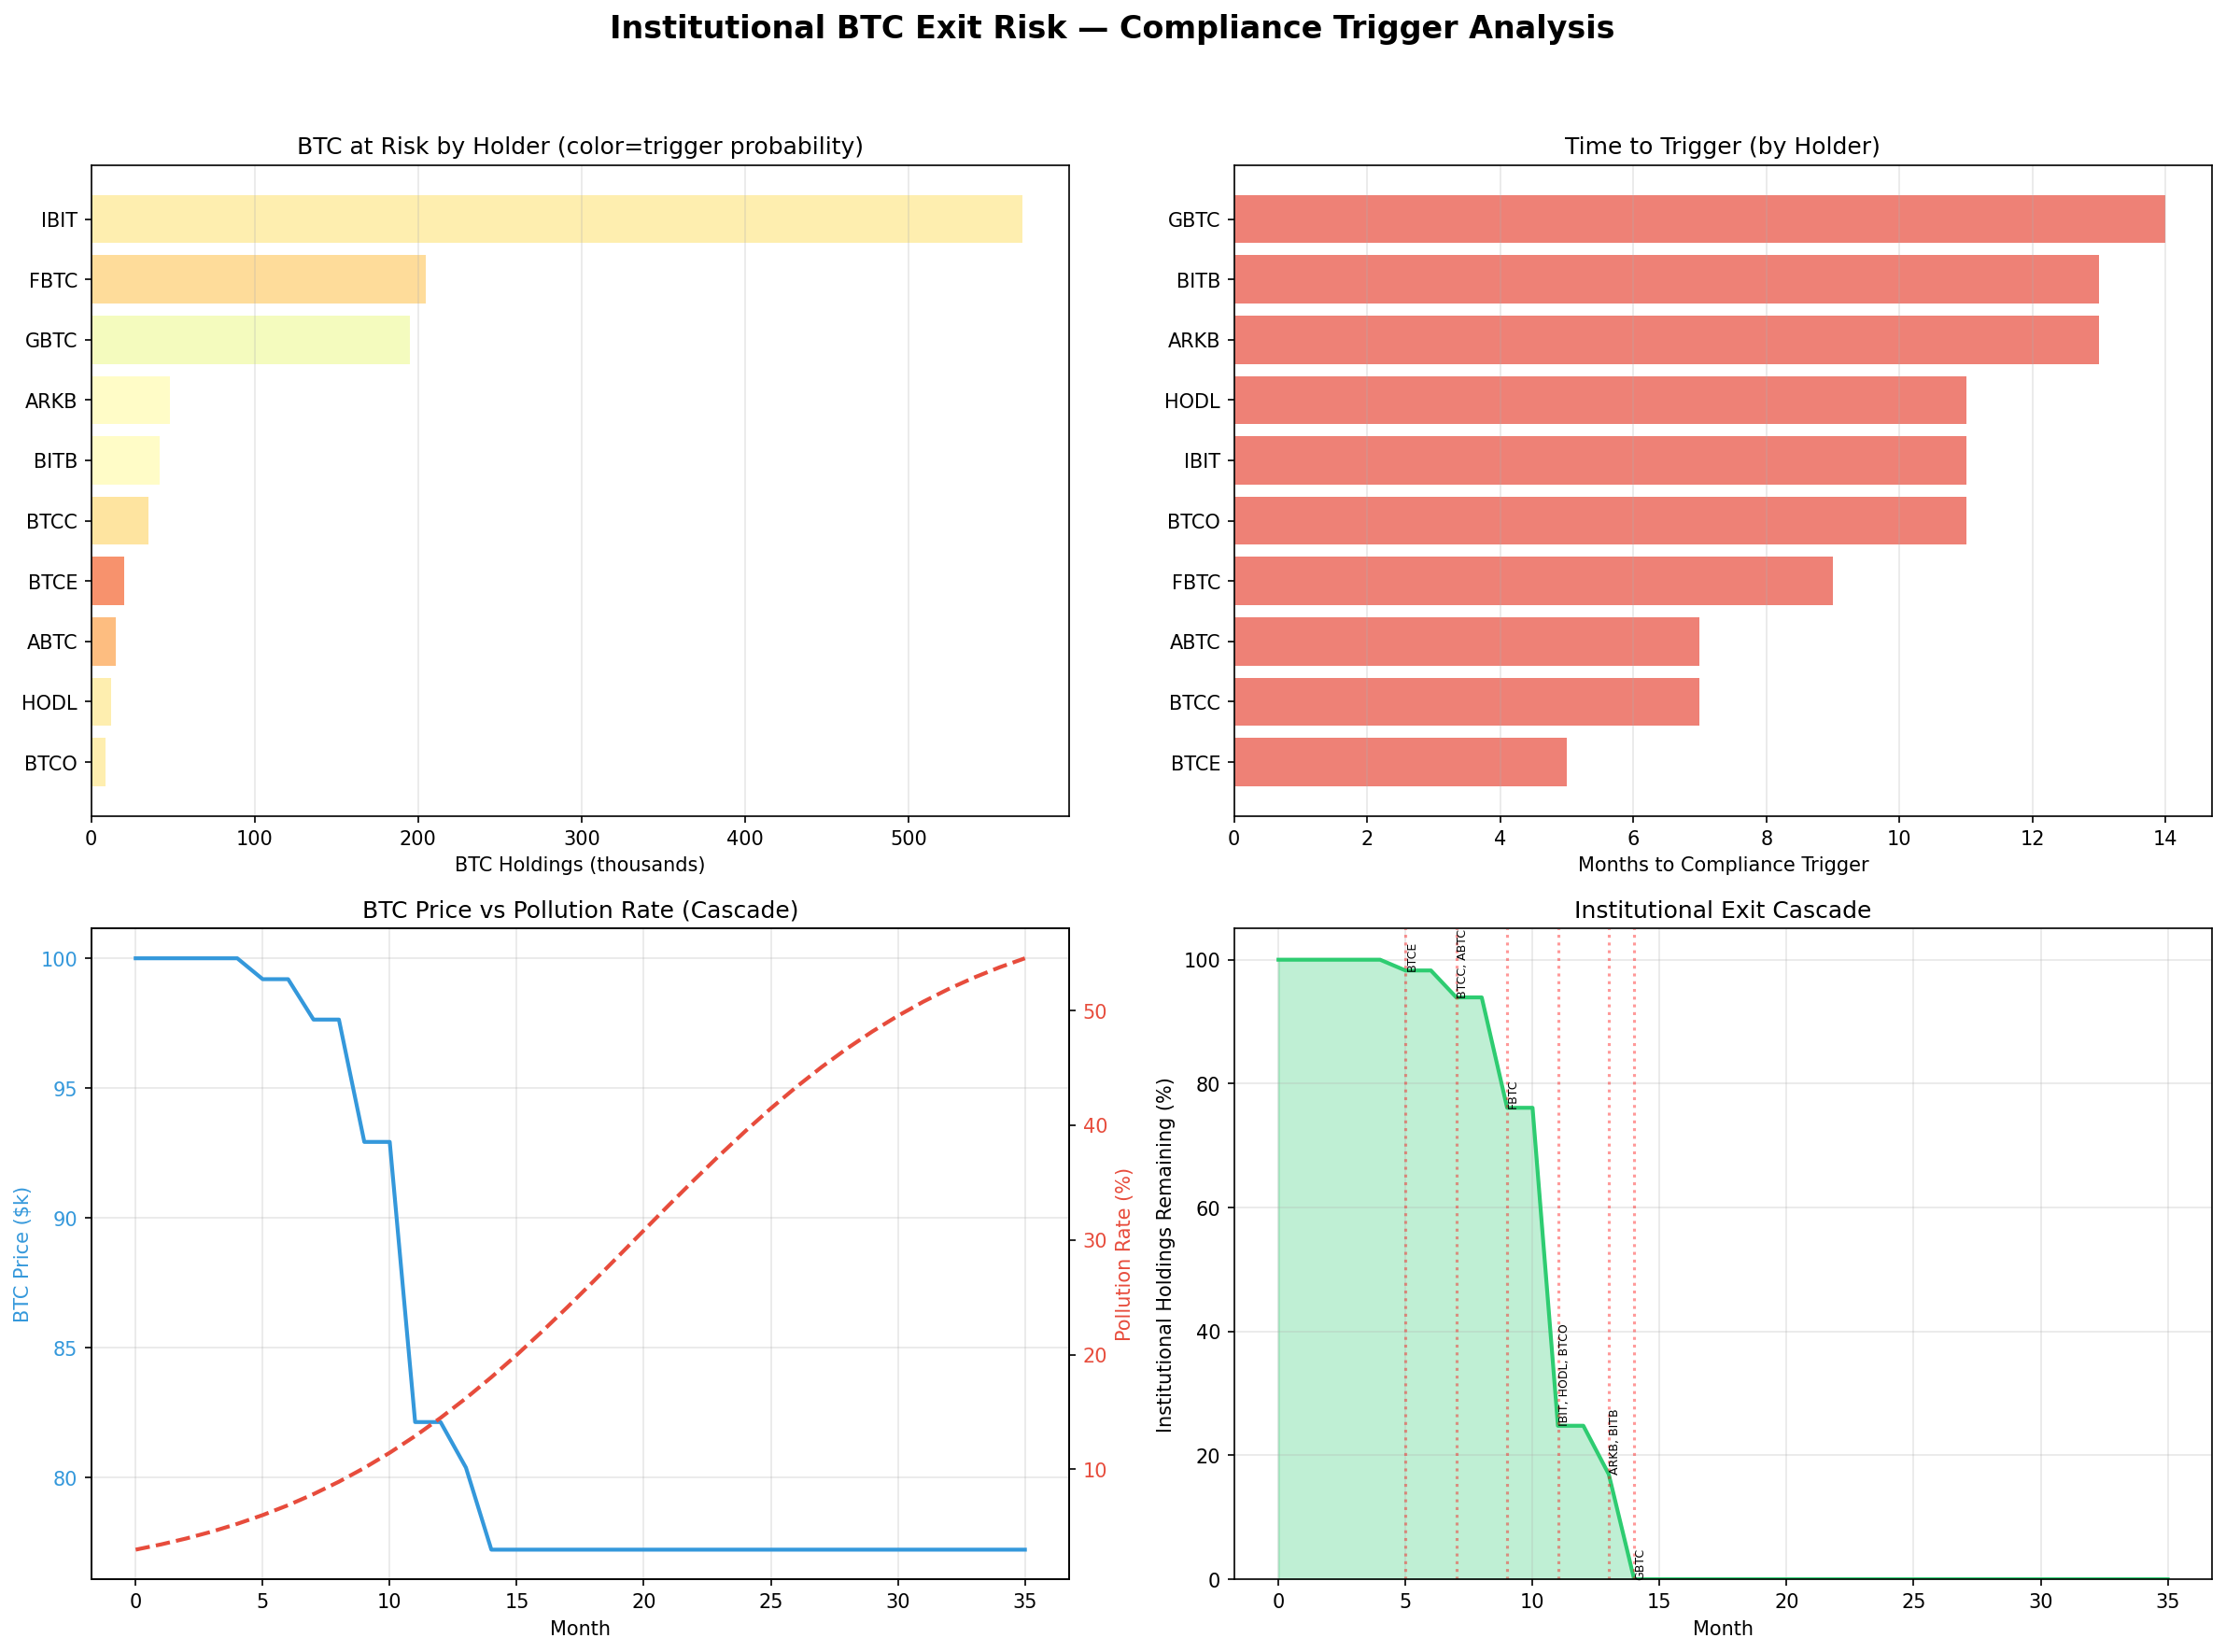
\includegraphics{../output/institutional_exit.png}

}

\caption{\label{fig-exit-cascade}Institutional exit cascade simulation
with Almgren-Chriss market impact. The figure presents four panels:
(top-left) a horizontal bar chart of BTC holdings by ETF issuer
color-coded by compliance trigger probability, with IBIT
(\textasciitilde570K BTC) holding the largest position at lower trigger
risk while smaller funds like BTCE face higher trigger probabilities;
(top-right) estimated months to compliance trigger for each holder,
ranging from approximately 4 to 14 months; (bottom-left) the simulated
cascade timeline showing cumulative BTC sold and the resulting price
trajectory under the Almgren-Chriss temporary and permanent impact
decomposition; (bottom-right) sensitivity of total market impact to
liquidation horizon, illustrating the classic execution-speed tradeoff
where faster exits (10 days) produce \textasciitilde3.5\% impact versus
\textasciitilde2.3\% for slower exits (90 days). The results demonstrate
that orderly liquidation substantially mitigates cascade risk compared
to naive forced-selling assumptions.}

\end{figure}

\hypertarget{sec-sensitivity}{%
\section{Sensitivity Analysis}\label{sec-sensitivity}}

\hypertarget{parameter-sensitivity}{%
\subsection{Parameter Sensitivity}\label{parameter-sensitivity}}

We test sensitivity to key model parameters:

\hypertarget{tbl-sensitivity}{}
\begin{longtable}[]{@{}
  >{\raggedright\arraybackslash}p{(\columnwidth - 6\tabcolsep) * \real{0.2500}}
  >{\raggedright\arraybackslash}p{(\columnwidth - 6\tabcolsep) * \real{0.2500}}
  >{\raggedright\arraybackslash}p{(\columnwidth - 6\tabcolsep) * \real{0.2500}}
  >{\raggedright\arraybackslash}p{(\columnwidth - 6\tabcolsep) * \real{0.2500}}@{}}
\caption{\label{tbl-sensitivity}Parameter sensitivity analysis.
Permanent impact (\(\gamma\)) and temporary impact (\(\eta\)) show the
highest sensitivity at ±40\% and ±30\% respectively, identifying them as
priority targets for empirical calibration.}\tabularnewline
\toprule\noalign{}
\begin{minipage}[b]{\linewidth}\raggedright
Parameter
\end{minipage} & \begin{minipage}[b]{\linewidth}\raggedright
Base Value
\end{minipage} & \begin{minipage}[b]{\linewidth}\raggedright
Range Tested
\end{minipage} & \begin{minipage}[b]{\linewidth}\raggedright
Impact on Key Output
\end{minipage} \\
\midrule\noalign{}
\endfirsthead
\toprule\noalign{}
\begin{minipage}[b]{\linewidth}\raggedright
Parameter
\end{minipage} & \begin{minipage}[b]{\linewidth}\raggedright
Base Value
\end{minipage} & \begin{minipage}[b]{\linewidth}\raggedright
Range Tested
\end{minipage} & \begin{minipage}[b]{\linewidth}\raggedright
Impact on Key Output
\end{minipage} \\
\midrule\noalign{}
\endhead
\bottomrule\noalign{}
\endlastfoot
DAA speed (\(\alpha\)) & 0.3 & {[}0.1, 0.5{]} & ±15\% on stabilized
degradation score \\
Energy share estimate & 0.6 & {[}0.5, 0.7{]} & ±8\% on breakeven
prices \\
Fee pushback reference (\(f_0\)) & 100 sat/vB & {[}50, 200{]} & ±20\% on
pollution saturation \\
Temporary impact (\(\eta\)) & 0.10 & {[}0.05, 0.20{]} & ±30\% on cascade
peak temporary impact \\
Permanent impact (\(\gamma\)) & 0.05 & {[}0.02, 0.10{]} & ±40\% on
cascade cumulative impact \\
Pollution weight allocation & See Section~\ref{sec-content-pollution} &
±50\% per weight & ±15\% on pollution probability \\
\end{longtable}

\hypertarget{key-sensitivities}{%
\subsection{Key Sensitivities}\label{key-sensitivities}}

The model is most sensitive to:

\begin{enumerate}
\def\labelenumi{\arabic{enumi}.}
\tightlist
\item
  \textbf{Almgren-Chriss coefficients} (\(\eta\), \(\gamma\)): These
  determine cascade severity. Empirical calibration from BTC-specific
  market microstructure data would significantly improve reliability.
\item
  \textbf{Fee pushback reference level}: Determines how effectively the
  fee market self-regulates pollution. Historical fee data could
  calibrate this more precisely.
\item
  \textbf{DAA speed}: Affects how quickly the network stabilizes after
  miner capitulation. The real DAA is a step function (every 2016
  blocks), while we use continuous smoothing.
\end{enumerate}

\hypertarget{robustness}{%
\subsection{Robustness}\label{robustness}}

Results are qualitatively robust across parameter ranges: the Nakamoto
Coefficient of 3 is a structural fact, fee-market pushback always
dampens pollution (only magnitude varies), and the DAA always provides
stabilizing feedback. The quantitative outputs should be interpreted as
order-of-magnitude estimates rather than point predictions.

\hypertarget{sec-discussion}{%
\section{Discussion}\label{sec-discussion}}

\hypertarget{interconnected-risks}{%
\subsection{Interconnected Risks}\label{interconnected-risks}}

The four risk vectors form feedback loops:

\begin{itemize}
\tightlist
\item
  Miner capitulation → reduced hashrate → increased concentration →
  lower censorship resistance
\item
  Content pollution → compliance triggers → institutional exit → price
  decline → miner capitulation
\item
  \textbf{Stabilizing}: Price decline → miner exit → difficulty
  adjustment → reduced breakeven → fewer exits
\item
  \textbf{Stabilizing}: Pollution pressure → fee increase → inscription
  pushback → reduced pollution
\end{itemize}

\hypertarget{limitations-1}{%
\subsection{Limitations}\label{limitations-1}}

\begin{itemize}
\tightlist
\item
  \textbf{Static vs.~dynamic}: While we add DAA feedback to miner stress
  and fee-market dynamics to pollution, the models remain largely
  open-loop. A full agent-based model (ABM) with coupled feedback across
  all four modules is left for future work.
\item
  \textbf{Pool hashrate ≠ censorship power}: Stratum V2 and pool-hopping
  dynamics significantly complicate censorship analysis
  (\protect\hyperlink{ref-cong2021}{Cong et al., 2021};
  \protect\hyperlink{ref-vernetti2023}{Vernetti, 2023}).
\item
  \textbf{ETF compliance triggers are speculative}: The pollution
  thresholds and compliance strictness parameters are estimated, not
  derived from actual compliance frameworks. ETFs hold UTXOs via
  custodians --- block content may be legally irrelevant unless OFAC
  sanctions specific addresses.
\item
  \textbf{Market impact calibration}: The Almgren-Chriss parameters
  (\(\eta\), \(\gamma\)) are calibrated to rough empirical estimates.
  BTC-specific market microstructure research, including time-varying
  market efficiency analysis (\protect\hyperlink{ref-noda2020}{Noda,
  2020}), would improve precision. Additionally, daily trading volume is
  assumed constant at \$30B, but Makarov \& Schoar
  (\protect\hyperlink{ref-makarov2020}{2020}) show that volume and
  market depth shrink substantially during systemic crashes ---
  precisely when institutional exits would occur --- amplifying realized
  market impact beyond our baseline estimates.
\item
  \textbf{Tracked miners represent \textasciitilde25\% of network}:
  Private miners with different cost structures are extrapolated,
  introducing uncertainty.
\item
  \textbf{DAA epoch stretch under mass capitulation}: When significant
  hashrate (e.g.~50\%) capitulates, block times lengthen proportionally
  (from \textasciitilde10 to \textasciitilde20 minutes), stretching the
  2016-block DAA adjustment window from \textasciitilde14 to
  \textasciitilde28 calendar days. Our exponential smoothing with
  constant time steps masks this real-time dilation effect,
  underestimating the duration of economic stress on surviving miners
  before difficulty relief arrives.
\end{itemize}

\hypertarget{miner-to-aihpc-pivot}{%
\subsection{Miner-to-AI/HPC Pivot}\label{miner-to-aihpc-pivot}}

A significant structural trend is the pivot of Bitcoin mining companies
toward AI and high-performance computing (HPC) hosting. TeraWulf (WULF)
has partnered with Google Cloud to repurpose mining infrastructure for
AI workloads, while Core Scientific (CORZ) has secured a major hosting
contract with CoreWeave, a GPU cloud provider.

This pivot has important implications for our miner stress model
(Section~\ref{sec-miner-stress}):

\begin{itemize}
\tightlist
\item
  \textbf{Reduced BTC-dependency}: Miners with diversified AI/HPC
  revenue streams have effectively lower breakeven prices for their
  Bitcoin mining operations, as fixed infrastructure costs are partially
  covered by non-BTC income. This makes them more resilient to BTC price
  declines.
\item
  \textbf{Hashrate concentration dynamics}: As diversified miners are
  less likely to capitulate during price downturns, the miners most
  vulnerable to capitulation are increasingly the \textbf{pure-play BTC
  miners} without alternative revenue. This could paradoxically increase
  hashrate concentration during stress events, as only the largest, most
  diversified operations survive.
\item
  \textbf{Reduced death-spiral risk}: The AI pivot provides an economic
  floor for mining infrastructure value independent of BTC price,
  further dampening the already self-correcting capitulation dynamics
  described in Section~\ref{sec-miner-stress}.
\end{itemize}

\hypertarget{implications-for-investors}{%
\subsection{Implications for
Investors}\label{implications-for-investors}}

\begin{itemize}
\tightlist
\item
  The DAA provides stronger resilience than static analysis suggests ---
  ``death spiral'' scenarios are partially self-correcting
\item
  Fee-market dynamics provide a natural ceiling on content pollution,
  reducing institutional compliance risk
\item
  Concentration risk (Nakamoto Coefficient = 3) remains the most
  structurally concerning finding
\item
  Institutional exit cascade risk is real but likely produces smaller,
  more gradual impact than naive models suggest
\end{itemize}

\hypertarget{implications-for-bitcoin-governance}{%
\subsection{Implications for Bitcoin
Governance}\label{implications-for-bitcoin-governance}}

\begin{itemize}
\tightlist
\item
  Stratum V2 adoption should be monitored as a key indicator of true
  censorship resistance
\item
  Geographic diversification of mining is a higher priority than raw
  hashrate growth
\item
  The fee market is a more effective regulator of block space usage than
  protocol-level restrictions
\end{itemize}

\hypertarget{sec-conclusion}{%
\section{Conclusion}\label{sec-conclusion}}

Our quantitative analysis reveals that Bitcoin's PoW security model
faces significant, interconnected vulnerabilities across mining
economics, network centralization, content pollution, and institutional
adoption. However, endogenous stabilization mechanisms --- particularly
the Difficulty Adjustment Algorithm and fee-market dynamics --- provide
meaningful resilience that static analyses miss.

The Nakamoto Coefficient of 3 and geographic concentration remain the
most structurally concerning findings, as these reflect market structure
rather than protocol design and are not self-correcting through
endogenous mechanisms.

These findings quantify the risk landscape to enable informed
decision-making by investors, regulators, and protocol developers. All
models and data are open-source for reproducibility and further
research.

\hypertarget{sec-future}{%
\section{Future Work}\label{sec-future}}

\begin{itemize}
\tightlist
\item
  Full agent-based model (ABM) with coupled feedback across all four
  risk vectors
\item
  Integration of real-time data feeds for continuous monitoring
\item
  Stratum V2 adoption tracking and its impact on effective Nakamoto
  Coefficient
\item
  Empirical calibration of Almgren-Chriss parameters from BTC market
  microstructure data
\item
  Extension to other PoW networks (Litecoin, Dogecoin, Kaspa)
\item
  Game-theoretic modeling of miner-pool strategic interactions
\item
  Regulatory scenario analysis across jurisdictions
\end{itemize}

\hypertarget{references}{%
\section*{References}\label{references}}
\addcontentsline{toc}{section}{References}

\hypertarget{refs}{}
\begin{CSLReferences}{1}{0}
\leavevmode\vadjust pre{\hypertarget{ref-almgren2001}{}}%
Almgren, R., \& Chriss, N. (2001). Optimal execution of portfolio
transactions. \emph{Journal of Risk}, \emph{3}(2), 5--39.

\leavevmode\vadjust pre{\hypertarget{ref-amihud2002}{}}%
Amihud, Y. (2002). Illiquidity and stock returns: Cross-section and
time-series effects. \emph{Journal of Financial Markets}, \emph{5}(1),
31--56.

\leavevmode\vadjust pre{\hypertarget{ref-bouchaud2008}{}}%
Bouchaud, J.-P., Farmer, J. D., \& Lillo, F. (2008). How markets slowly
digest changes in supply and demand. In T. Hens \& K. R. Schenk-Hoppé
(Eds.), \emph{Handbook of financial markets: Dynamics and evolution}
(pp. 57--160). North-Holland.

\leavevmode\vadjust pre{\hypertarget{ref-carter2023}{}}%
Carter, N., \& Jeng, L. (2023). Ordinals and the fee market. \emph{Coin
Metrics State of the Network}.

\leavevmode\vadjust pre{\hypertarget{ref-chen2025}{}}%
Chen, Y. et al. (2025). Bitcoin {ETF} impact on futures markets.
\emph{International Review of Financial Analysis}.

\leavevmode\vadjust pre{\hypertarget{ref-cong2021}{}}%
Cong, L. W., He, Z., \& Li, J. (2021). Decentralized mining in
centralized pools. \emph{Review of Financial Studies}, \emph{34}(3),
1191--1235.

\leavevmode\vadjust pre{\hypertarget{ref-easley2019}{}}%
Easley, D., O'Hara, M., \& Basu, S. (2019). From mining to markets: The
role of {Bitcoin} transaction fees. \emph{Journal of Financial
Economics}, \emph{134}(1), 91--109.

\leavevmode\vadjust pre{\hypertarget{ref-gencer2018}{}}%
Gencer, A. E. et al. (2018). Decentralization in {Bitcoin} and
{Ethereum} networks. \emph{Proceedings of NDSS 2018}.

\leavevmode\vadjust pre{\hypertarget{ref-judmayer2021}{}}%
Judmayer, A. et al. (2021). Estimating the cost of a 51\% attack.
\emph{Financial Cryptography and Data Security (FC 2021)}.

\leavevmode\vadjust pre{\hypertarget{ref-makarov2020}{}}%
Makarov, I., \& Schoar, A. (2020). Trading and arbitrage in
cryptocurrency markets. \emph{Journal of Financial Economics},
\emph{135}(2), 293--319.

\leavevmode\vadjust pre{\hypertarget{ref-nakamoto2008}{}}%
Nakamoto, S. (2008). \emph{Bitcoin: A peer-to-peer electronic cash
system}. \url{https://bitcoin.org/bitcoin.pdf}.

\leavevmode\vadjust pre{\hypertarget{ref-noda2020}{}}%
Noda, A. (2020). On the evolution of cryptocurrency market efficiency.
\emph{Applied Economics Letters}, \emph{28}(6), 433--439.

\leavevmode\vadjust pre{\hypertarget{ref-prat2021}{}}%
Prat, J., \& Walter, B. (2021). An equilibrium model of the market for
{Bitcoin} mining. \emph{Journal of Political Economy}, \emph{129}(8),
2415--2452.

\leavevmode\vadjust pre{\hypertarget{ref-vernetti2023}{}}%
Vernetti, F. (2023). \emph{Stratum {V2}: The next generation protocol
for pooled mining}. Braiins Technical Documentation.

\leavevmode\vadjust pre{\hypertarget{ref-wendl2025}{}}%
Wendl, M. et al. (2025). Bitcoin {Ordinals}: A systematic analysis.
\emph{Journal of The British Blockchain Association (JBBA)}.

\end{CSLReferences}

\hypertarget{sec-appendix-a}{%
\section*{Appendix A: Technical Implementation}\label{sec-appendix-a}}
\addcontentsline{toc}{section}{Appendix A: Technical Implementation}

All models are implemented in Python 3.12+ and available at:
\url{https://github.com/IngoGiebel/powsec-models}

\hypertarget{dependencies}{%
\subsection*{Dependencies}\label{dependencies}}
\addcontentsline{toc}{subsection}{Dependencies}

\begin{verbatim}
pandas, numpy, matplotlib, scipy, yfinance, requests
\end{verbatim}

\hypertarget{reproduction}{%
\subsection*{Reproduction}\label{reproduction}}
\addcontentsline{toc}{subsection}{Reproduction}

\begin{Shaded}
\begin{Highlighting}[]
\ExtensionTok{pip}\NormalTok{ install }\AttributeTok{{-}r}\NormalTok{ requirements.txt}
\ExtensionTok{python}\NormalTok{ miner\_stress.py}
\ExtensionTok{python}\NormalTok{ content\_pollution.py}
\ExtensionTok{python}\NormalTok{ hashrate\_concentration.py}
\ExtensionTok{python}\NormalTok{ institutional\_exit.py}
\end{Highlighting}
\end{Shaded}

Output: \texttt{output/} directory with PNG visualizations and CSV data
files.

\hypertarget{sec-appendix-b}{%
\section*{Appendix B: Model Parameters}\label{sec-appendix-b}}
\addcontentsline{toc}{section}{Appendix B: Model Parameters}

\hypertarget{b.1-miner-stress-parameters}{%
\subsection*{B.1 Miner Stress
Parameters}\label{b.1-miner-stress-parameters}}
\addcontentsline{toc}{subsection}{B.1 Miner Stress Parameters}

\hypertarget{tbl-miner-params}{}
\begin{longtable}[]{@{}
  >{\raggedright\arraybackslash}p{(\columnwidth - 4\tabcolsep) * \real{0.3333}}
  >{\raggedright\arraybackslash}p{(\columnwidth - 4\tabcolsep) * \real{0.3333}}
  >{\raggedright\arraybackslash}p{(\columnwidth - 4\tabcolsep) * \real{0.3333}}@{}}
\caption{\label{tbl-miner-params}Miner stress model parameters sourced
from blockchain data and industry reports.}\tabularnewline
\toprule\noalign{}
\begin{minipage}[b]{\linewidth}\raggedright
Parameter
\end{minipage} & \begin{minipage}[b]{\linewidth}\raggedright
Value
\end{minipage} & \begin{minipage}[b]{\linewidth}\raggedright
Source
\end{minipage} \\
\midrule\noalign{}
\endfirsthead
\toprule\noalign{}
\begin{minipage}[b]{\linewidth}\raggedright
Parameter
\end{minipage} & \begin{minipage}[b]{\linewidth}\raggedright
Value
\end{minipage} & \begin{minipage}[b]{\linewidth}\raggedright
Source
\end{minipage} \\
\midrule\noalign{}
\endhead
\bottomrule\noalign{}
\endlastfoot
Network hashrate & 850 EH/s & Blockchain.com, mid-2025 \\
Block reward & 3.125 BTC & Post-April 2024 halving \\
Energy share estimate & 60\% of mining revenue & CoinShares mining
reports \\
DAA adjustment speed & \(\alpha = 0.3\) & Smoothing approximation \\
Logistic steepness & \(k = 5.0\) & Calibrated for gradual transition \\
\end{longtable}

\hypertarget{b.2-content-pollution-parameters}{%
\subsection*{B.2 Content Pollution
Parameters}\label{b.2-content-pollution-parameters}}
\addcontentsline{toc}{subsection}{B.2 Content Pollution Parameters}

\hypertarget{tbl-pollution-params}{}
\begin{longtable}[]{@{}
  >{\raggedright\arraybackslash}p{(\columnwidth - 4\tabcolsep) * \real{0.3333}}
  >{\raggedright\arraybackslash}p{(\columnwidth - 4\tabcolsep) * \real{0.3333}}
  >{\raggedright\arraybackslash}p{(\columnwidth - 4\tabcolsep) * \real{0.3333}}@{}}
\caption{\label{tbl-pollution-params}Content pollution model parameters
governing inscription density, fee pushback, and flagging
sensitivity.}\tabularnewline
\toprule\noalign{}
\begin{minipage}[b]{\linewidth}\raggedright
Parameter
\end{minipage} & \begin{minipage}[b]{\linewidth}\raggedright
Value
\end{minipage} & \begin{minipage}[b]{\linewidth}\raggedright
Source
\end{minipage} \\
\midrule\noalign{}
\endfirsthead
\toprule\noalign{}
\begin{minipage}[b]{\linewidth}\raggedright
Parameter
\end{minipage} & \begin{minipage}[b]{\linewidth}\raggedright
Value
\end{minipage} & \begin{minipage}[b]{\linewidth}\raggedright
Source
\end{minipage} \\
\midrule\noalign{}
\endhead
\bottomrule\noalign{}
\endlastfoot
Max block size & 4.0 MB (weight) & Bitcoin protocol (SegWit) \\
Fee pushback reference & \(f_0 = 100\) sat/vB & Empirical median during
high-fee periods \\
Density normalization & 100 inscriptions/block & Observed peak
density \\
Flag sensitivity & 50× scaling & 0.2\% flagged ≈ significant \\
\end{longtable}

\hypertarget{b.3-hashrate-concentration-parameters}{%
\subsection*{B.3 Hashrate Concentration
Parameters}\label{b.3-hashrate-concentration-parameters}}
\addcontentsline{toc}{subsection}{B.3 Hashrate Concentration Parameters}

\hypertarget{tbl-hashrate-params}{}
\begin{longtable}[]{@{}
  >{\raggedright\arraybackslash}p{(\columnwidth - 4\tabcolsep) * \real{0.3333}}
  >{\raggedright\arraybackslash}p{(\columnwidth - 4\tabcolsep) * \real{0.3333}}
  >{\raggedright\arraybackslash}p{(\columnwidth - 4\tabcolsep) * \real{0.3333}}@{}}
\caption{\label{tbl-hashrate-params}Hashrate concentration data sources
for mining pool shares, geographic distribution, and regulatory
compliance estimates.}\tabularnewline
\toprule\noalign{}
\begin{minipage}[b]{\linewidth}\raggedright
Parameter
\end{minipage} & \begin{minipage}[b]{\linewidth}\raggedright
Value
\end{minipage} & \begin{minipage}[b]{\linewidth}\raggedright
Source
\end{minipage} \\
\midrule\noalign{}
\endfirsthead
\toprule\noalign{}
\begin{minipage}[b]{\linewidth}\raggedright
Parameter
\end{minipage} & \begin{minipage}[b]{\linewidth}\raggedright
Value
\end{minipage} & \begin{minipage}[b]{\linewidth}\raggedright
Source
\end{minipage} \\
\midrule\noalign{}
\endhead
\bottomrule\noalign{}
\endlastfoot
Pool data & Mid-2025 estimates & BTC.com, mempool.space \\
Geographic data & CBECI estimates & Cambridge Centre for Alternative
Finance \\
KYC/Gov compliance multipliers & 0.1×--2.0× & Expert estimate
(sensitivity needed) \\
\end{longtable}

\hypertarget{b.4-institutional-exit-parameters}{%
\subsection*{B.4 Institutional Exit
Parameters}\label{b.4-institutional-exit-parameters}}
\addcontentsline{toc}{subsection}{B.4 Institutional Exit Parameters}

\hypertarget{tbl-exit-params}{}
\begin{longtable}[]{@{}lll@{}}
\caption{\label{tbl-exit-params}Institutional exit cascade parameters
including temporary and permanent price impact coefficients calibrated
to empirical estimates.}\tabularnewline
\toprule\noalign{}
Parameter & Value & Source \\
\midrule\noalign{}
\endfirsthead
\toprule\noalign{}
Parameter & Value & Source \\
\midrule\noalign{}
\endhead
\bottomrule\noalign{}
\endlastfoot
Temporary impact \(\eta\) & 0.10 & Calibrated to empirical estimates \\
Permanent impact \(\gamma\) & 0.05 & Calibrated to empirical
estimates \\
Daily BTC volume & \$30B & CoinGecko average, mid-2025 \\
ETF holdings data & Mid-2025 estimates & ETF issuer reports \\
\end{longtable}

\begin{center}\rule{0.5\linewidth}{0.5pt}\end{center}

\emph{This research was conducted with AI assistance from Claude
(Anthropic) for analysis coordination and code generation, and reviewed
by Google Gemini 3 Deep Think for mathematical validation.}



\end{document}
